%Version 3 October 2023
% See section 11 of the User Manual for version history
%
%%%%%%%%%%%%%%%%%%%%%%%%%%%%%%%%%%%%%%%%%%%%%%%%%%%%%%%%%%%%%%%%%%%%%%
%%                                                                 %%
%% Please do not use \input{...} to include other tex files.       %%
%% Submit your LaTeX manuscript as one .tex document.              %%
%%                                                                 %%
%% All additional figures and files should be attached             %%
%% separately and not embedded in the \TeX\ document itself.       %%
%%                                                                 %%
%%%%%%%%%%%%%%%%%%%%%%%%%%%%%%%%%%%%%%%%%%%%%%%%%%%%%%%%%%%%%%%%%%%%%

%%\documentclass[referee,sn-basic]{sn-jnl}% referee option is meant for double line spacing

%%=======================================================%%
%% to print line numbers in the margin use lineno option %%
%%=======================================================%%

%%\documentclass[lineno,sn-basic]{sn-jnl}% Basic Springer Nature Reference Style/Chemistry Reference Style

%%======================================================%%
%% to compile with pdflatex/xelatex use pdflatex option %%
%%======================================================%%

%%\documentclass[pdflatex,sn-basic]{sn-jnl}% Basic Springer Nature Reference Style/Chemistry Reference Style


%%Note: the following reference styles support Namedate and Numbered referencing. By default the style follows the most common style. To switch between the options you can add or remove “Numbered” in the optional parenthesis. 
%%The option is available for: sn-basic.bst, sn-vancouver.bst, sn-chicago.bst%  
 
%%\documentclass[sn-nature]{sn-jnl}% Style for submissions to Nature Portfolio journals
\documentclass[sn-basic]{sn-jnl}% Basic Springer Nature Reference Style/Chemistry Reference Style
% \documentclass[sn-mathphys-num]{sn-jnl}% Math and Physical Sciences Numbered Reference Style 
%%\documentclass[sn-mathphys-ay]{sn-jnl}% Math and Physical Sciences Author Year Reference Style
%%\documentclass[sn-aps]{sn-jnl}% American Physical Society (APS) Reference Style
%%\documentclass[sn-vancouver,Numbered]{sn-jnl}% Vancouver Reference Style
%%\documentclass[sn-apa]{sn-jnl}% APA Reference Style 
%%\documentclass[sn-chicago]{sn-jnl}% Chicago-based Humanities Reference Style

%%%% Standard Packages
%%<additional latex packages if required can be included here>

\usepackage{graphicx}%
\usepackage{multirow}%
\usepackage{amsmath,amssymb,amsfonts}%
\usepackage{amsthm}%
\usepackage{mathrsfs}%
\usepackage[title]{appendix}%
\usepackage{xcolor}%
\usepackage{textcomp}%
\usepackage{manyfoot}%
\usepackage{booktabs}%
\usepackage{algorithm}%
\usepackage{algorithmicx}%
\usepackage{algpseudocode}%
\usepackage{listings}%
\usepackage{tabularx}

\newcommand{\JH}[1]{\textcolor{blue}{[JH: #1]}}
%%%%

%%%%%=============================================================================%%%%
%%%%  Remarks: This template is provided to aid authors with the preparation
%%%%  of original research articles intended for submission to journals published 
%%%%  by Springer Nature. The guidance has been prepared in partnership with 
%%%%  production teams to conform to Springer Nature technical requirements. 
%%%%  Editorial and presentation requirements differ among journal portfolios and 
%%%%  research disciplines. You may find sections in this template are irrelevant 
%%%%  to your work and are empowered to omit any such section if allowed by the 
%%%%  journal you intend to submit to. The submission guidelines and policies 
%%%%  of the journal take precedence. A detailed User Manual is available in the 
%%%%  template package for technical guidance.
%%%%%=============================================================================%%%%

%% as per the requirement new theorem styles can be included as shown below
\theoremstyle{thmstyleone}%
\newtheorem{theorem}{Theorem}%  meant for continuous numbers
%%\newtheorem{theorem}{Theorem}[section]% meant for sectionwise numbers
%% optional argument [theorem] produces theorem numbering sequence instead of independent numbers for Proposition
\newtheorem{proposition}[theorem]{Proposition}% 
%%\newtheorem{proposition}{Proposition}% to get separate numbers for theorem and proposition etc.

\theoremstyle{thmstyletwo}%
\newtheorem{example}{Example}%
\newtheorem{remark}{Remark}%

\theoremstyle{thmstylethree}%
\newtheorem{definition}{Definition}%

\raggedbottom
%%\unnumbered% uncomment this for unnumbered level heads

\begin{document}

% \title{Scenario-based Motion Forecasting for Autonomous Vehicles: A Survey} 
\title{Motion Forecasting for Autonomous Vehicles: A Survey} 

%%=============================================================%%
%% GivenName	-> \fnm{Joergen W.}
%% Particle	-> \spfx{van der} -> surname prefix
%% FamilyName	-> \sur{Ploeg}
%% Suffix	-> \sfx{IV}
%% \author*[1,2]{\fnm{Joergen W.} \spfx{van der} \sur{Ploeg} 
%%  \sfx{IV}}\email{iauthor@gmail.com}
%%=============================================================%%

% \author[1]{\fnm{First} \sur{Jianxin Shi}}\email{shijx@buaa.edu.cn}
% \equalcont{These authors contributed equally to this work.}
% \author[1]{\fnm{Second} \sur{Jinhao Chen}}\email{chenjh24@buaa.edu.cn}
% \equalcont{These authors contributed equally to this work.}
% \author*[2]{\fnm{Third} \sur{Yuandong Wang}}\email{iiiauthor@gmail.com}

\author[1]{\sur{Jianxin Shi}}\email{shijx@buaa.edu.cn}
\equalcont{These authors contributed equally to this work.}
\author[1]{\sur{Jinhao Chen}}\email{chenjh24@buaa.edu.cn}
\equalcont{These authors contributed equally to this work.} 
\author*[2]{\sur{Yuandong Wang}}\email{wangyd@cnu.edu.cn}
\author[3]{\sur{Li Sun}}\email{ccesunli@ncepu.edu.cn}
\author[4]{\sur{Chunyang Liu}}\email{liuchunyang@didiglobal.com}
\author[4]{\sur{Wei Xiong}}\email{xiongwei@didiglobal.com}
\author[1]{\sur{Tianyu Wo}}\email{woty@buaa.edu.cn}


\affil[1]{\orgdiv{Beijing Advanced Innovation Center for Big Data and Brain Computing}, \orgname{Beihang University}, \orgaddress{\city{Beijing}, \postcode{100191}, \country{China}}}

\affil*[2]{\orgdiv{Information Engineering College}, \orgname{Capital Normal University}, \orgaddress{\city{Beijing}, \postcode{100048}, \country{China}}}

\affil[3]{\orgdiv{School of Control and Computer Engineering}, \orgname{North China Electric Power University}, \orgaddress{\city{Beijing}, \postcode{102206}, \country{China}}}

\affil[4]{\orgname{Didi Chuxing}, \orgaddress{\city{Beijing}, \postcode{100094}, \country{China}}}


% \affil[1]{\orgdiv{Beijing Advanced Innovation Center for Big Data and Brain Computing}, \orgname{Beihang University}, \orgaddress{\street{Street}, \city{Beijing}, \postcode{100191}, \state{State}, \country{China}}}

% \affil*[2]{\orgdiv{Department}, \orgname{Capital Normal University}, \orgaddress{\street{Street}, \city{Beijing}, \postcode{100048}, \state{State}, \country{China}}}

% \affil[3]{\orgdiv{Department}, \orgname{North China Electric Power University}, \orgaddress{\street{Street}, \city{Beijing}, \postcode{102206}, \state{State}, \country{China}}}

% \affil[4]{\orgdiv{Department}, \orgname{Didi Chuxing}, \orgaddress{\street{Street}, \city{Beijing}, \postcode{}, \state{State}, \country{China}}}



%%==================================%%
%% Sample for unstructured abstract %%
%%==================================%%

\abstract{In recent years, the field of autonomous driving has attracted increasingly significant public interest. Accurately forecasting the future behavior of various traffic participants is essential for the decision-making of Autonomous Vehicles (AVs). 
% In this paper, we focus on motion forecasting for AVs under the scenario-based setting. 
In this paper, we focus on both scenario-based and perception-based motion forecasting for AVs.
We propose a formal problem formulation for motion forecasting and summarize the main challenges confronting this area of research. We also detail representative datasets and evaluation metrics pertinent to this field. Furthermore, this study classifies recent research into two main categories: supervised learning and self-supervised learning, reflecting the evolving paradigms in both scenario-based and perception-based motion forecasting. In the context of supervised learning, we thoroughly examine and analyze each key element of the methodology. For self-supervised learning, we summarize commonly adopted techniques. The paper concludes and discusses potential research directions, aiming to propel progress in this vital area of AV technology.}

%%================================%%
%% Sample for structured abstract %%
%%================================%%

% \abstract{\textbf{Purpose:} The abstract serves both as a general introduction to the topic and as a brief, non-technical summary of the main results and their implications. The abstract must not include subheadings (unless expressly permitted in the journal's Instructions to Authors), equations or citations. As a guide the abstract should not exceed 200 words. Most journals do not set a hard limit however authors are advised to check the author instructions for the journal they are submitting to.
% 
% \textbf{Methods:} The abstract serves both as a general introduction to the topic and as a brief, non-technical summary of the main results and their implications. The abstract must not include subheadings (unless expressly permitted in the journal's Instructions to Authors), equations or citations. As a guide the abstract should not exceed 200 words. Most journals do not set a hard limit however authors are advised to check the author instructions for the journal they are submitting to.
% 
% \textbf{Results:} The abstract serves both as a general introduction to the topic and as a brief, non-technical summary of the main results and their implications. The abstract must not include subheadings (unless expressly permitted in the journal's Instructions to Authors), equations or citations. As a guide the abstract should not exceed 200 words. Most journals do not set a hard limit however authors are advised to check the author instructions for the journal they are submitting to.
% 
% \textbf{Conclusion:} The abstract serves both as a general introduction to the topic and as a brief, non-technical summary of the main results and their implications. The abstract must not include subheadings (unless expressly permitted in the journal's Instructions to Authors), equations or citations. As a guide the abstract should not exceed 200 words. Most journals do not set a hard limit however authors are advised to check the author instructions for the journal they are submitting to.}

\keywords{Deep Learning, Autonomous Driving, Motion Forecasting, Vehicle Trajectory Prediction.}

%%\pacs[JEL Classification]{D8, H51}

%%\pacs[MSC Classification]{35A01, 65L10, 65L12, 65L20, 65L70}

\maketitle

\section{Introduction}
Motion Forecasting is vital in the functionality of autonomous driving systems. It assists these vehicles in planning their forthcoming actions and mitigates the risk of accidents. 
% This survey is dedicated to motion forecasting within the context of autonomous vehicles. The primary inputs for motion forecasting are the state information and road structure information of target agents, both provided by the perception module and surrounding agents. Through a comprehensive analysis of both the environmental semantic information and the target's intention information, motion forecasting involves making intention predictions for all perceived agents and forecasting their trajectories for a certain period into the future. 
This survey addresses motion forecasting in autonomous vehicles, focusing on the two main approaches: Scenario-based Motion Forecasting and Perception-based Motion Forecasting.

\textbf{Scenario-based Motion Forecasting} predicts future states of traffic agents (TAs) by analyzing past states and relevant environmental context, such as high-definition maps (HDMaps) and the historical states of surrounding agents (SAs). This approach emphasizes structured, predefined inputs like agents' locations and HDMaps, intentionally excluding raw sensor data like RGB images, LiDAR point clouds, or semantic segmentation maps. By limiting input features to these structured elements, scenario-based forecasting models achieve a focused analysis of the traffic environment and agent interactions.

\textbf{Perception-based Motion Forecasting}, on the other hand, directly utilizes raw perception data, including camera images, LiDAR point clouds, and other sensor outputs, to predict agents' future trajectories. This approach bypasses intermediate feature engineering steps, allowing the model to learn relevant representations directly from raw data. Perception-based methods aim to leverage richer environmental cues, making them suitable for scenarios where comprehensive scene understanding is crucial.

Multiple approaches have been suggested to tackle the prediction problem, including physics-based models, rule-based models, and deep learning-based models. 
Among these, \textbf{physics-based models} \cite{xie2017vehicle} offer a distinct approach by utilizing physical principles to predict vehicle trajectories over the short term. These models incorporate factors such as current position, acceleration, and turn rate to estimate future movements. To elaborate, 
Constant Velocity (CV) models~\cite{scholler2020constant} operate under the assumption that a vehicle maintains its speed in the same direction without acceleration. Similarly, 
Constant Acceleration (CA) models~\cite{polychronopoulos2007sensor} predict movement based on unchanging acceleration in the current direction. 
For scenarios involving both constant speed and constant turn rate, Constant Turn Rate and Velocity (CTRV) models~\cite{lytrivis2008cooperative} are applied. 
Meanwhile, Constant Turn Rate and Acceleration (CTRA) models~\cite{barth2008will} anticipate that a vehicle will maintain both its acceleration and turn rate consistently. Implementing these physics-based approaches is relatively straightforward, requiring minimal computing resources. However, these models have limitations, notably their overlook of environmental factors and interactions with other agents. As a result, while they are efficient for short-term predictions in uncomplicated environments, their applicability is limited by the complexity of the environment and the presence of multiple dynamic agents, underlining the necessity for more sophisticated models in certain contexts. 
\textbf{Rule-based models}~\cite{liu2022probabilistic,qingkai2020lightweight} leverage known traffic rules and human prior knowledge, predicting the future trajectory of vehicles with a structured approach. Initially, models confirm the current state of target agents, a task typically handled by the tracking module that outputs to the prediction module. Following this, the current lane of the vehicle is determined based on its present position and direction. Subsequently, the future lane is predicted according to the vehicle's current state. The final step involves generating the trajectory based on two scenarios: maintaining the current lane or changing lanes. The simplicity and intuitiveness of this method stem from the use of predefined rules, which also contribute to its low computational complexity, ease of adjustment, and reliability. These advantages make rule-based models adapt to various scenarios. However, the inflexibility and limited generalization capabilities of rule-based models pose significant challenges. Since the rules are hard-coded, adapting to new and unseen scenes becomes problematic. Furthermore, capturing and quantifying complex scenes or non-linear interactions is difficult, escalating the complexity of maintaining such a rule-based approach as the number of unforeseen scenarios increases. 
\textbf{Deep learning-based models} have significantly advanced motion forecasting for the long term as Figure~\ref{Figure 1}, leveraging the capabilities of sequential neural networks to extract complex patterns and relationships from extensive datasets. 

\begin{figure}[H]
    \centering
    \includegraphics[width=\textwidth]{Fig1.eps}
    \caption{The increasing trend within the research community is evidenced by the growing number of articles on Google Scholar that include the keywords "Autonomous Driving" and "Vehicle Motion Forecasting" published between 2019 and 2024.}
    \label{Figure 1}
\end{figure}

% Have greatly improved long-term motion forecasting by utilizing sequential neural networks to extract complex patterns and relationships from extensive datasets.
These models excel at integrating a wide range of factors, including those related to physics, road conditions, and vehicle interactions, making them exceptionally adaptable to the intricate dynamics of traffic environments. Among the diverse approaches, RNN-based networks \cite{multipath,covernet}, Graph-based networks \cite{vectornet,tnt,densetnt,lanegcn,lanercnn}, and Transformer-based networks \cite{2021scene-transformer,2021AutoBot,2022multi-modal-transformer,2022hivt} stand out, each offering unique strengths in analyzing temporal and spatial data complexities. All these methodologies are based on supervised learning, which has traditionally dominated the field. However, the challenge of acquiring high-precision, labeled trajectory data suitable for autonomous driving prediction has prompted a shift toward innovative solutions. In the last two years, self-supervised learning has emerged as a promising direction in the realm of autonomous vehicles. 
This approach aims to mitigate the scarcity of high-quality data by using strategies such as data augmentation \cite{Pretram,azevedo2022exploiting,li2023pre} to enhance and diversify available datasets. These self-supervised techniques represent a proactive response to the limitations of traditional supervised learning, offering a pathway to refine motion forecasting despite the hurdles posed by data constraints.

This survey aims to provide a comprehensive review of the latest research in motion forecasting for AVs, covering the general pipelines of both scenario-based and perception-based methods. The structure of the survey is outlined as follows: Section 2 introduces the problem formulation of trajectory prediction, laying out the foundational concepts. Section 3 delves into the main challenges faced in the motion forecasting task, highlighting key areas of difficulty. Section 4 offers a comparison of commonly used motion forecasting datasets and elaborates on the corresponding three levels of evaluation metrics. Sections 5 and 6 are dedicated to discussing the motion forecasting sequence network, with Section 5 focusing on approaches based on supervised learning and Section 6 on those utilizing self-supervised learning. The survey concludes with Section 7, where we present our conclusion and explore potential directions for future research, as Figure~\ref{Figure 2}.
\begin{figure}[H]
    \centering
    \includegraphics[width=\textwidth]{Fig2.eps}
    \caption{Overview of motion forecasting methodologies, challenges, and future directions for autonomous vehicle trajectory prediction.}
    \label{Figure 2}
\end{figure}

% Our survey aims to provide a comprehensive review of the latest research in motion forecasting for autonomous vehicles, with a specific focus on resolving issues within the prediction problem pipeline.
% \vspace{-2ex}

\section{Problem Formulation}
% The goal of vehicle trajectory prediction is to predict the future states of target agents, \(T_{pred}\), given its past states \(T_{obs}\) and traffic scenes which consist of High Definition (HD) Maps, past states of surrounding traffic agents, \(T_{obs}\), etc.
This section introduces some important definitions and formally formulates the problem of motion forecasting. 
\subsection{Definitions}

% 2.1 Definitions
% {
% 2.1.1 Definitions of Traffic Participants
% 2.1.2 Input
% 2.1.3 Output
% }
% 2.2 Problem Formulation
% {
% 2.2.1 Scenario-based
% 2.2.2 Perception-based
% }

\subsubsection{Traffic Participants}

\indent\textbf{Target Agents (TAs).} Target Agents represent the objects that are crucial for analysis and prediction in autonomous vehicle systems. Their future behavior or trajectory is of utmost importance for the safe and efficient operation of autonomous vehicles.

\textbf{Ego Agent (EA).} Ego Agent refers to an autonomous vehicle whose behavior is influenced by its surrounding environment. This includes the behavior of TAs, road conditions, and other similar factors.

\textbf{Surrounding Agents (SAs).} Surrounding Agents refer to objects such as other vehicles, bicycles, pedestrians, and similar entities that can potentially impact the future behavior of TAs. Different studies use varied criteria for selecting SAs, depending on the specific assumptions underlying their models. 
The visualization of their relationship in the traffic scene is shown in Figure~\ref{Figure 3}. 

% \textbf{Past States of TAs.} For the target agent, its state in the past \(T_{obs}\) time is expressed as:
% \begin{equation}
% X_{TAs}=\{X_{target,t-T_{obs}},...,X_{target,t-1},X_{target,t}\},
% \end{equation}
% where \(X\) represents physical state characteristics of the target agent in the past \(T_{obs}\) time, such as the position, velocity, heading, yaw, etc.

\begin{figure}[H]
    \centering
    \includegraphics[width=0.5\textwidth]{Fig3.eps}
    \caption{Different types of traffic participants (agents).}
    \label{Figure 3}
\end{figure}


\subsubsection{Input Representation}

Motion forecasting can be divided based on different types of input data, each providing unique information that can enhance prediction accuracy. In this section, we review motion forecasting methods categorized by their input types: trajectory and HDMap data, Bird’s Eye View (BEV) representation, and raw perception data. Each category leverages distinct characteristics of the environment and agent dynamics, offering varied advantages in predicting future trajectories.


\textbf{Raw Perception Data.}
Raw perception data serves as an essential component in motion forecasting tasks, providing unprocessed sensor information directly from the environment. In the context of autonomous driving, this data typically comes from sensors like LiDAR, radar, and cameras, offering a richer and more detailed view of the surroundings compared to structured data like trajectories or HD maps. The raw perception data includes point clouds, visual images, and radar reflections, which capture both the static and dynamic aspects of the scene.

A point cloud, for instance, generated by LiDAR sensors, can be formalized as:
\begin{equation}
P = \{(x_{p1}, y_{p1}, z_{p1}, r_{p1}), \dots, (x_{pM}, y_{pM}, z_{pM}, r_{pM})\}
\end{equation} 
where \((x, y, z)\) represents the 3D position of each point in space, and \(r\) is the reflectance value indicating the intensity of the return signal. The number of points, \(M\), may vary based on the environment and the sensor’s resolution.

Similarly, camera images provide 2D pixel information, capturing visual elements such as road signs, obstacles, or pedestrians. This can be represented as a tensor:
\begin{equation}
I = \{(I_{r,g,b})_{w,h}\},
\end{equation}
where \(I_{r,g,b}\) denotes the RGB values for each pixel located at width \(w\) and height \(h\) of the image. Radar data, though less detailed than LiDAR or camera, can detect the velocity of objects with higher accuracy and provides valuable complementary information for forecasting.

Integrating raw perception data into motion forecasting models presents both challenges and opportunities. The high dimensionality and unstructured nature of raw sensor data require sophisticated feature extraction techniques, such as deep learning-based methods, to transform the data into a form suitable for trajectory prediction. Methods like voxelization of point clouds or the extraction of salient features from images are commonly used to handle these raw inputs.


\textbf{Scenario Representation.} For an autonomous vehicle motion prediction problem, the scene representation consists of two parts: High Definition (HD) Map and the states of SAs during past \(T_{obs}\) time.
The mathematical representation of HDMap can be formalized as:
\begin{gather}
    HDMap = \{Lanes=\{(x_{11},y_{11},Attr_1,Lights_1(t)),...,\notag\\
              (x_{l1},y_{l1},Attr_l,Lights_l(t)),...,\notag\\(x_{L1},y_{L1},Attr_L,Lights_L(t))\};\notag\\
              Lights_l(t)=\{state_{t1}(t),...,state_{tT_{obs}}(t)\} \},
\end{gather}
where \((x,y\)) and \(Attr\) represent the position and attribute of the lane segment (such as intersection or not, speed limit or not), respectively. \(L\) is the number of lane segments. \(Lights_l\) represents the change in traffic light status for lane segment $l$, which is a discrete variable containing three elements: "Red", "Yellow", and "Green".

For surrounding agents, their state in the past \(T_{obs}\) time can be formalized as:
\begin{equation}
X_{SAs}=\{X_{1,t-T_{obs}},...,X_{N,t}\},
\end{equation}
where \(X\) represents physical state characteristics of \(N\) surrounding agents in the past \(T_{obs}\) time, such as the position, velocity, heading, etc.

\textbf{BEV Representation.}
% Bird's Eye View (BEV) representation is another powerful input modality used in motion forecasting. BEV provides a top-down, two-dimensional representation of the scene, capturing the positions of agents and road elements from an overhead perspective. This method simplifies the scene geometry by projecting 3D data into a 2D plane, while still retaining crucial spatial relationships between objects and agents.
Bird’s Eye View (BEV) representations convert raw sensor data, such as LiDAR point clouds or camera images, into a 2D grid format that simplifies the processing and modeling of spatial relationships. This transformation enables motion forecasting models to efficiently capture interactions between agents and their environment, as well as improve the prediction of future trajectories.

The BEV representation can be formalized as:
\begin{equation}
BEV = \{(x_{bev}, y_{bev}, f(x_{bev}, y_{bev}))\},
\end{equation}
where \((x_{bev}, y_{bev})\) are the 2D coordinates in the BEV plane, and \(f(x_{bev}, y_{bev})\) represents various features extracted from the input data, such as occupancy, velocity, or semantic information (e.g., lane markings, drivable areas). The grid size and resolution of the BEV representation determine the trade-off between computational efficiency and prediction accuracy.

BEV representations have gained popularity due to their ability to encode complex spatial information and facilitate the modeling of multi-agent interactions. Many state-of-the-art motion forecasting models leverage BEV to predict the future paths of both the ego vehicle and surrounding agents in a unified manner.



\subsubsection{Prediction Types}

% \textbf{Intentions}

\textbf{Marginal Trajectory Prediction.} In the marginal prediction case, the trajectories of TAs do not affect each other, the prediction goal can be formalized as:
\begin{equation}
Output\_Marginal_{T_{pred}}=p(s_1)p(s_2)...p(s_n),
\end{equation}
where \(p(s_i)\) represents the predicted trajectory distribution of agent \(i\) in the future, which is related to the historical states of agent \(i\), the historical states of agent \(j\), and the HDMap.

\textbf{Joint Multi-Agent Prediction.}Unlike marginal trajectory prediction, joint multi-agent prediction is more complex and essential as it requires predicting the future trajectories of multiple vehicles while considering their mutual interactions and influences, as shown in Figure~\ref{Figure 4}. This prediction method integrates the states and intentions of all vehicles, better reflecting the dynamic changes in real traffic environments. 
\begin{figure}[H]
    \centering
    \includegraphics[width=\textwidth]{Fig4.eps}
    \caption{The relationship between marginal prediction and joint multi-agent prediction. The main difference between them is that the former has a single $TA$; The latter has multiple $TAs$.}
    \label{Figure 4}
\end{figure}

In the joint prediction case, compared with marginal prediction, the interdependencies between TAs' future behavior can be captured, and the prediction goal is:
\begin{equation}
Output\_Joint_{T_{pred}}=p(s_1,s_2,...,s_n),
\end{equation}
Compared to the marginal prediction, \(p(s_i)\) is also related to the future prediction trajectory of agent \(j\). 

\subsection{Problem Formulation}

Motion forecasting pipelines can generally be categorized into two main approaches based on the data flow and processing stages: \textbf{Scenario-based Motion Forecasting} and \textbf{Perception-based Motion Forecasting}. 
The pipelines for these two approaches are illustrated in Figure \ref{Figure 5}.
% The pipelines for these two approaches are illustrated in Figure \ref{fig:scenario-based} and Figure \ref{fig:perception-prediction}, respectively.


\begin{figure}[H]
    \centering
    \includegraphics[width=\textwidth]{Fig5.eps}
    \caption{Comparison of scenario-based and perception-based motion forecasting pipelines in autonomous driving.}
    \label{Figure 5}
\end{figure}


% \begin{figure}[H]
%     \centering
%     \includegraphics[width=\textwidth]{img/scenario-based.pdf}
%     \caption{The pipeline of scenario-based motion forecasting task.}
%     \label{fig:scenario-based}
% \end{figure}

% \begin{figure}[H]
%     \centering
%     \includegraphics[width=0.9\textwidth]{img/perception-prediction.pdf}
%     \caption{The pipeline of end-to-end motion forecasting task.}
%     \label{fig:perception-prediction}
% \end{figure} 

% \JH{move to Methods}

\subsubsection{Scenario-based Motion Forecasting}
The primary objective of motion forecasting is to predict the future states of TAs, considering their past states as well as the surrounding traffic scenes. These traffic scenes encompass various elements, including HDMaps, past states of SAs, and other relevant factors. In contrast to survey \cite{teeti2022vision-based-survey} focusing on vision-based prediction models in AVs, the scenario-based motion forecasting model restricts its input features to agents' location information and HDMaps. These models specifically exclude other types of data such as RGB images, Lidar point clouds, semantic segmentation maps, and any other additional data. Considering these specific inclusions and exclusions, the overall input for these models can be formalized as:
% \vspace{-2ex}
\begin{equation}
Input_{T_{obs}}=\{X_{TAs},HDMap,X_{SAs},Others\},
\end{equation}
where \(Others\) represents the other information such as traffic congestion of the current lane, lighting status of SAs, and the planned trajectory of EA, etc.

The forecasting process then predicts the future trajectories of the target agents based on this structured input. The predicted trajectory for a target agent can be formalized as:
\begin{equation}
\hat{X}_{TA} = \{(x_{ta,t+1}, y_{ta,t+1}), (x_{ta,t+2}, y_{ta,t+2}), ..., (x_{ta,t+T}, y_{ta,t+T})\},
\end{equation}
where \((x_{ta,t+i}, y_{ta,t+i})\) represents the position of the target agent at each future time step \(t+i\), and \(T\) is the prediction horizon.

% To train the model, a common objective is to minimize the error between the predicted trajectory \(\hat{X}_{TA}\) and the ground truth trajectory \(X^*_{TA}\), using a loss function like mean squared error (MSE):
% \[
% \mathcal{L} = \sum_{i=1}^{T} || \hat{X}_{TA,i} - X^{*}_{TA,i} ||^2.
% \]

By focusing on structured inputs such as HD maps and past agent states, scenario-based motion forecasting aims to leverage the explicit representations of the environment and agent dynamics to achieve accurate trajectory predictions.


\subsubsection{Perception-based Motion Forecasting} 
Perception-based motion forecasting refers to the approach of directly predicting the future trajectories of agents from raw perception data, such as camera images, LiDAR point clouds, and other raw sensor data. without the need for artificially designed intermediate features or steps. 

Mathematically, the end-to-end motion forecasting process can be described as learning a function \(f\), which maps the raw perception data \(Z_{t}\) (e.g., LiDAR point clouds or camera images) to the future trajectories \(X_{t+T}\) of the agents:
\begin{equation}
f: Z_{t} \to X_{t+T},
\end{equation}
where \(Z_{t} = \{Z_{LiDAR}, Z_{camera}, Z_{radar}, ...\}\) represents the raw sensor data at time \(t\), and \(X_{t+T}\) is the predicted trajectory of the target agent(s) over the future time horizon \(T\).

The predicted trajectory \(X_{t+T}\) can be further formalized as a sequence of future states over \(T\) time steps:
\begin{equation}
X_{t+T} = \{X_{t+1}, X_{t+2}, ..., X_{t+T}\},
\end{equation}
where each future state \(X_{t+i}\) typically includes information such as position, velocity, and heading of the agent at time \(t+i\). The learning objective for the model is to minimize the prediction error between the ground truth future trajectory \(X^{*}_{t+T}\) and the predicted trajectory \(X_{t+T}\), using a loss function such as mean squared error (MSE):
\begin{equation}
\mathcal{L} = \sum_{i=1}^{T} || X_{t+i} - X^{*}_{t+i} ||^2.
\end{equation}

By training the model end-to-end with this objective, it learns to capture the intricate dynamics of the environment and agent interactions, directly from the raw perception data, enabling accurate and robust motion forecasting.

% The primary benefit of end-to-end motion forecasting is its ability to learn a direct mapping from raw sensor data (such as LiDAR point clouds, camera images, or radar signals) to future trajectories.
By bypassing intermediate steps like handcrafted feature extraction or external map information, these models can potentially avoid the error propagation often seen in staged pipelines. Furthermore, end-to-end approaches allow the model to learn implicit representations of the environment, agents, and their interactions from raw data, potentially leading to richer and more nuanced predictions. 

% \section{Related Work}


\textbf{Class-Incremental Learning (CIL)} necessitates a model that can continuously learn new classes while retaining knowledge of previously learned ones \cite{dohare2024loss,cao2023retentive,zhou2023revisiting,zhou2024continual}, which can be roughly divided into several categories. 
Regularization-based methods incorporate explicit regularization terms into the loss function to balance the weights assigned to new and old tasks \cite{kirkpatrick2017overcoming,aljundi2018memory,wang2022continual,li2017learning}.
Replay-based methods address the problem of catastrophic forgetting by replaying data from previous classes during the training of new ones. This can be achieved by either directly using complete data from old classes \cite{lopez2017gradient,riemer2018learning,cha2021co2l,wang2022foster} or by generating samples \cite{shin2017continual,zhu2022self}, such as employing GANs to synthesize samples from previous classes \cite{cong2020gan,liu2020generative}.
Dynamic network methods adapt to new classes by adjusting the network structure, such as adding neurons or layers, to maintain sensitivity to previously learned knowledge while acquiring new tasks. This approach allows the model's capacity to expand based on task requirements, improving its ability to manage knowledge accumulation in CIL \cite{wang2022coscl,wang2023incorporating,aljundi2017expert,ostapenko2021continual}.
Recently, CIL methods based on pre-trained models (PTMs)
\cite{cao2023retentive,chen2022adaptformer,zhou2024continual} have demonstrated promising results.
Prompt-based methods utilize prompt tuning \cite{jia2022visual} to facilitate lightweight updates to PTMs. By keeping the pre-trained weights frozen, these methods preserve the generalizability of PTMs, thereby mitigating the forgetting in CIL \cite{smith2023coda,wang2022dualprompt,NEURIPS2023_d9f8b5ab,wang2022learning,wang2022dualprompt,smith2023coda,li2024learning}. 
Model mixture-based methods mitigate forgetting by saving models during training and integrating them through model ensemble or model merge techniques \cite{gao2023unified,wang2023isolation,wang2024hierarchical,zheng2023preventing,zhou2023learning,zhou2024expandable}.
Prototype-based methods draw from the concept of representation learning \cite{ye2017learning}, leveraging the robust representation capabilities of PTMs for classification with NCM classifiers \cite{panos2023first,zhou2023revisiting,mcdonnell2024ranpac}.

\textbf{The Order in CIL} remains a significant and unresolved challenge \cite{wang2024comprehensive}. APD \cite{yoon2019scalable} effectively addresses the problem of CF by decomposing model parameters into task-shared and sparse task-specific components, thereby enhancing the model's robustness to changes in class order. HALRP \cite{li2024hessian}, on the other hand, simulates parameter conversion in continuous tasks by applying low-rank approximation to task-adaptive parameters at each layer of the neural network, thereby improving the model's order robustness. However, the optimization strategies employed by these methods are confined to the network architecture itself and do not fundamentally resolve the underlying issues.
Recent theoretical analyses of CIL \cite{lin2023theory,shan2024order,bell2022effect,wu2021curriculum} indicate that prioritizing the learning of tasks (or classes) with lower similarity enhances the model's generalization and resistance to forgetting. Building on these theories, we conducted further research and developed corresponding methods in the following sections.


% \input{2.1.Definitions of Traffic Participants}
% \input{2.2.Input Representation}
% \input{2.2.Problem Formulation}
% \input{2.4.Prediction Tasks}

% \documentclass{standalone}
%\usetikzlibrary{...}
\usepackage{tikz}
\begin{document}
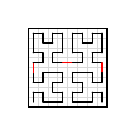
\begin{tikzpicture}
\tikzstyle{helperline} = [lightgray!60!white, line width=0.1mm];
\draw[line cap=round][helperline] (-0.0,0.125) -- (1.0,0.125);
\draw[line cap=round][helperline] (-0.0,0.25) -- (1.0,0.25);
\draw[line cap=round][helperline] (-0.0,0.375) -- (1.0,0.375);
\draw[line cap=round][helperline] (-0.0,0.5) -- (1.0,0.5);
\draw[line cap=round][helperline] (-0.0,0.625) -- (1.0,0.625);
\draw[line cap=round][helperline] (-0.0,0.75) -- (1.0,0.75);
\draw[line cap=round][helperline] (-0.0,0.875) -- (1.0,0.875);
\draw[line cap=round][helperline]  (0.125,1.0) -- (0.125,-0.0);
\draw[line cap=round][helperline]  (0.25,1.0) -- (0.25,-0.0);
\draw[line cap=round][helperline]  (0.375,1.0) -- (0.375,-0.0);
\draw[line cap=round][helperline]  (0.5,1.0) -- (0.5,-0.0);
\draw[line cap=round][helperline]  (0.625,1.0) -- (0.625,-0.0);
\draw[line cap=round][helperline]  (0.75,1.0) -- (0.75,-0.0);
\draw[line cap=round][helperline]  (0.875,1.0) -- (0.875,-0.0);
\draw[line cap=round]  (0,1) rectangle (1,0);
\draw[line cap=round] (0.0625, 0.0625) -- (0.0625, 0.1875);
\draw[line cap=round] (0.0625, 0.1875) -- (0.1875, 0.1875);
\draw[line cap=round] (0.1875, 0.1875) -- (0.1875, 0.0625);
\draw[line cap=round] (0.1875, 0.0625) -- (0.3125, 0.0625);
\draw[line cap=round] (0.3125, 0.0625) -- (0.4375, 0.0625);
\draw[line cap=round] (0.4375, 0.0625) -- (0.4375, 0.1875);
\draw[line cap=round] (0.4375, 0.1875) -- (0.3125, 0.1875);
\draw[line cap=round] (0.3125, 0.1875) -- (0.3125, 0.3125);
\draw[line cap=round] (0.3125, 0.3125) -- (0.4375, 0.3125);
\draw[line cap=round] (0.4375, 0.3125) -- (0.4375, 0.4375);
\draw[line cap=round] (0.4375, 0.4375) -- (0.3125, 0.4375);
\draw[line cap=round] (0.3125, 0.4375) -- (0.1875, 0.4375);
\draw[line cap=round] (0.1875, 0.4375) -- (0.1875, 0.3125);
\draw[line cap=round] (0.1875, 0.3125) -- (0.0625, 0.3125);
\draw[line cap=round] (0.0625, 0.3125) -- (0.0625, 0.4375);
\draw[line cap=round,red] (0.0625, 0.4375) -- (0.0625, 0.5625);
\draw[line cap=round] (0.0625, 0.5625) -- (0.1875, 0.5625);
\draw[line cap=round] (0.1875, 0.5625) -- (0.1875, 0.6875);
\draw[line cap=round] (0.1875, 0.6875) -- (0.0625, 0.6875);
\draw[line cap=round] (0.0625, 0.6875) -- (0.0625, 0.8125);
\draw[line cap=round] (0.0625, 0.8125) -- (0.0625, 0.9375);
\draw[line cap=round] (0.0625, 0.9375) -- (0.1875, 0.9375);
\draw[line cap=round] (0.1875, 0.9375) -- (0.1875, 0.8125);
\draw[line cap=round] (0.1875, 0.8125) -- (0.3125, 0.8125);
\draw[line cap=round] (0.3125, 0.8125) -- (0.3125, 0.9375);
\draw[line cap=round] (0.3125, 0.9375) -- (0.4375, 0.9375);
\draw[line cap=round] (0.4375, 0.9375) -- (0.4375, 0.8125);
\draw[line cap=round] (0.4375, 0.8125) -- (0.4375, 0.6875);
\draw[line cap=round] (0.4375, 0.6875) -- (0.3125, 0.6875);
\draw[line cap=round] (0.3125, 0.6875) -- (0.3125, 0.5625);
\draw[line cap=round] (0.3125, 0.5625) -- (0.4375, 0.5625);
\draw[line cap=round,red] (0.4375, 0.5625) -- (0.5625, 0.5625);
\draw[line cap=round] (0.5625, 0.5625) -- (0.6875, 0.5625);
\draw[line cap=round] (0.6875, 0.5625) -- (0.6875, 0.6875);
\draw[line cap=round] (0.6875, 0.6875) -- (0.5625, 0.6875);
\draw[line cap=round] (0.5625, 0.6875) -- (0.5625, 0.8125);
\draw[line cap=round] (0.5625, 0.8125) -- (0.5625, 0.9375);
\draw[line cap=round] (0.5625, 0.9375) -- (0.6875, 0.9375);
\draw[line cap=round] (0.6875, 0.9375) -- (0.6875, 0.8125);
\draw[line cap=round] (0.6875, 0.8125) -- (0.8125, 0.8125);
\draw[line cap=round] (0.8125, 0.8125) -- (0.8125, 0.9375);
\draw[line cap=round] (0.8125, 0.9375) -- (0.9375, 0.9375);
\draw[line cap=round] (0.9375, 0.9375) -- (0.9375, 0.8125);
\draw[line cap=round] (0.9375, 0.8125) -- (0.9375, 0.6875);
\draw[line cap=round] (0.9375, 0.6875) -- (0.8125, 0.6875);
\draw[line cap=round] (0.8125, 0.6875) -- (0.8125, 0.5625);
\draw[line cap=round] (0.8125, 0.5625) -- (0.9375, 0.5625);
\draw[line cap=round,red] (0.9375, 0.5625) -- (0.9375, 0.4375);
\draw[line cap=round] (0.9375, 0.4375) -- (0.9375, 0.3125);
\draw[line cap=round] (0.9375, 0.3125) -- (0.8125, 0.3125);
\draw[line cap=round] (0.8125, 0.3125) -- (0.8125, 0.4375);
\draw[line cap=round] (0.8125, 0.4375) -- (0.6875, 0.4375);
\draw[line cap=round] (0.6875, 0.4375) -- (0.5625, 0.4375);
\draw[line cap=round] (0.5625, 0.4375) -- (0.5625, 0.3125);
\draw[line cap=round] (0.5625, 0.3125) -- (0.6875, 0.3125);
\draw[line cap=round] (0.6875, 0.3125) -- (0.6875, 0.1875);
\draw[line cap=round] (0.6875, 0.1875) -- (0.5625, 0.1875);
\draw[line cap=round] (0.5625, 0.1875) -- (0.5625, 0.0625);
\draw[line cap=round] (0.5625, 0.0625) -- (0.6875, 0.0625);
\draw[line cap=round] (0.6875, 0.0625) -- (0.8125, 0.0625);
\draw[line cap=round] (0.8125, 0.0625) -- (0.8125, 0.1875);
\draw[line cap=round] (0.8125, 0.1875) -- (0.9375, 0.1875);
\draw[line cap=round] (0.9375, 0.1875) -- (0.9375, 0.0625);
\end{tikzpicture}
\end{document}

\section{Challenges}
% In the domain of autonomous driving, motion forecasting for vehicles is relatively more predictable than that of other vulnerable traffic participants, such as pedestrians and cyclists. This predictability stems from vehicles' adherence to established traffic rules and specific dynamic constraints. However, motion forecasting for vehicles remains a complex task due to the dynamic nature of traffic environments.
In the domain of autonomous driving, motion forecasting for TAs is very supportive of the EA's next move. However, accurate motion forecasting for TAs remains a challenging task due to the complexity and flexible traffic environment.
%In the domain of autonomous driving, motion forecasting for vehicles is very supportive of the autonomous one's next move. However, accurate motion forecasting for vehicles remains a challenging task due to the complexity and flexible traffic environment.

% \textbf{The complexity of road environment.}
\textbf{Fusion of road information.} 
% HD Maps are integral to autonomous driving systems and comprise detailed features surpassing those of traditional navigation maps, achieving accuracies up to the centimeter scale. These maps are synthesized using an array of sensors, including radar, lidar, and cameras, which facilitate the capture and assembly of requisite data. 
% HD Maps with centimeter-level accuracy are very necessary to autonomous driving systems, which comprise detailed features surpassing those of traditional navigation maps. These maps are collected through various sensors, including radar, lidar, and cameras which facilitate the capture of abundant information. 
% Essential to autonomous vehicles, HD Maps encompass comprehensive road section data and intricate lane information for each segment. The geometry of these lanes significantly influences vehicles' behavior. Consequently, motion forecasting models for vehicles devoid of lane geometry considerations exhibit constrained performance in complex traffic scenarios.
% For the advancement of the autonomous driving field, researchers collect road information using a series of sensors, after processing and manual verification, the information contributes to the construction of HD Maps. HD Maps provide more detailed features and achieve centimeter-level accuracy, offering important information for vehicle behavior prediction. However, the lack of unified standards in HD Maps' data formats and content poses significant challenges. How to establish data alignment and association between HD Maps and agents' trajectories, and effectively integrate this information in vehicle behavior prediction is a huge challenge.
To advance the autonomous driving field, researchers utilize more detailed features and achieve centimeter-level accuracy for vehicle behavior prediction by constructing HDMaps. 
These HDMaps provide rich contextual information, such as lane boundaries, traffic signs, and road geometry, which are crucial for making precise and reliable predictions. However, the absence of unified standards in HDMaps' data formats and content poses significant challenges. How to establish data alignment and association between HDMaps and agents' trajectories, and effectively integrate this information in vehicle behavior prediction is a huge challenge. 



% \textbf{The interdependence of vehicle behavior.} 
\textbf{Dynamic interactions between different vehicles.} 
The influence of road environments on vehicle behavior is static, whereas the interaction between SAs and TAs is dynamic and uncertain, posing significant challenges in capturing this complex interplay. For instance, a vehicle's decision to turn right at an intersection involves interacting with the static environment of the right-turn lane. However, the dynamic and variable nature of interactions between SAs and TAs adds complexity, making the analysis and interpretation of these interaction patterns significantly more challenging.

\textbf{Multimodality of vehicle behavior.} 
In autonomous driving, understanding the behaviors of TAs and SAs is critical due to their inherent multimodality, meaning a single historical trajectory can lead to multiple potential future trajectories. 
The combination of an agent's trajectory with road information provides valuable insights into the driver's style, especially their familiarity with specific road sections. A deeper analysis of the agent's historical movement patterns enables the identification of various possible future behaviors. Consequently, an effective motion forecasting module in an autonomous driving system should be able to recognize all these potential future behaviors. This capability is essential to ensure the system operates reliably and safely.

\textbf{Lack of interpretability.}
% Many existing motion forecasting models adopt data-driven methodologies to learn trajectory distributions, which often leads to a lack of interpretability in the decision-making processes of traffic participants. 
Many existing motion forecasting models adopt data-driven methodologies to learn trajectory distributions. While these approaches can achieve high levels of accuracy by leveraging large datasets, they often result in a lack of interpretability in the decision-making processes of traffic participants. This black-box nature makes it challenging to understand or explain why a model predicts certain behaviors, which is crucial for both safety and trust in autonomous systems. Moreover, the reliance on purely data-driven techniques can lead to overfitting specific scenarios or biases present in the data, potentially reducing the generalizability and robustness of the models in diverse and dynamic real-world environments. As a result, there is an increasing need for approaches that not only predict motion accurately but also offer clear insights into the underlying factors influencing these predictions. 

% resulting in a lack of interpretability in the decision-making processes of traffic participants.


% \section{The Proposed Method: GDDSG}\label{sec4}
\begin{figure*}
    \centering
    \includegraphics[width=\linewidth]{figures/framework.pdf}
    \caption{Illustration of The Overall Framework. [best view in color]}
    \label{fig: framework}
\end{figure*}
\textbf{Overview.} \autoref{fig: framework} provides an overview of our proposed method. 
Using task \( t \) as an example, we begin by projecting all training samples into an embedding space utilizing a pre-trained backbone. In this space, we compute the centroids for each class. Next, we evaluate whether a new centroid \( \mathbf{c}_i \) should be integrated into an existing class group \( G_j \).
If \( \mathbf{c}_i \) is dissimilar to all classes within \( G_j \), it is added to the group. If it is similar to any class in an existing group, it remains unassigned.
For unassigned centroids, we construct new similarity graphs (SimGraphs) based on their pairwise similarities. We then apply graph coloring theory to these SimGraphs, forming new class groups by clustering dissimilar categories together.
Finally, we update the NCM-based classifier with all class groups, facilitating efficient model updates with minimal computational overhead.

\subsection{Class Grouping Based on Similarity}

\autoref{Corollary: cor} provides guidance for constructing a sequence of dissimilar tasks. A key idea is to dynamically assign each new class to a group during CIL, ensuring that the similarity between the new class and other classes within the group is minimized. This approach helps maintain the robustness of each group's incremental learning process to the order of tasks. For each group, a separate adapter can be trained, and the results from different adapters can be merged during prediction to enhance the model's overall performance. 

In a given CIL task sequence, we organize the classes into several groups. The group list is denoted as \( G = [G_1, \dots, G_k] \), where each \( G_i \) represents a distinct group of classes. For a specified task \( t \) and each class \( C \in CLS^t \), our objective is to assign class \( C \) to an optimal group \( G^* \), ensuring that the new class is dissimilar to all existing classes in that group.

To achieve this objective, we first define the similarity between classes.
The similarity between any two classes, \( CLS_i \) and \( CLS_j \), is determined using an adaptive similarity threshold \( \eta_{i,j} \).
This threshold is computed based on the mean distance between the training samples of each class and their respective centroids in a learned embedding space, as shown below:

\begin{align}
    \eta_{i,j} = \max [
    & \frac{\sum_{k = 1}^{|X^t|} \mathbb{I}(y^t_k = i) \, d(h(x_k^t), \mathbf{c_i}) }{\sum_{k = 1}^{|X^t|} \mathbb{I}(y^t_k = i)}, \nonumber \\
    & \frac{\sum_{k = 1}^{|X^t|} \mathbb{I}(y^t_k = j) \, d(h(x_k^t), \mathbf{c_j}) }{\sum_{k = 1}^{|X^t|} \mathbb{I}(y^t_k = j)} 
    ],
\end{align}
where \( \mathbf{x}^{(t)} \) denotes the t-th task instance, \( h(\cdot) \) is the feature extraction function defined in Equation \autoref{eq: feature}, \( d: \mathcal{X} \times \mathcal{X} \to \mathbb{R}^+ \) specifies the distance metric space, \( \mathbb{I}(\cdot) \) represents the characteristic function, and the class centroid \( \mathbf{c}_i \in \mathbb{R}^d \) is computed as \( \mathbf{c}_i = \frac{1}{|C_i|} \sum_{x_j \in C_i} \mathbf{x}_j \).


Building upon this framework, we define the condition under which two classes, \( CLS_i \) and \( CLS_j \), are considered dissimilar. Specifically, they are deemed dissimilar if the following condition holds:

\begin{equation}
    d(\mathbf{c_i}, \mathbf{c_j}) > \eta_{i,j}.
    \label{eq: sim}
\end{equation}

Thus, class \( C \) is assigned to group \( G^* \) only if it is dissimilar to all classes within \( G^* \), and \( G^* \) is the choice with the lowest average similarity:

\begin{equation}
    G^* = \arg\min_{G} \frac{1}{|G|} \sum_{C' \in G} d(C, C').
\end{equation}

This approach is consistent with the principles outlined in \autoref{Corollary: cor} and ensures the robustness of the model across the entire task sequence.


\subsection{Graph-Driven Class Grouping}

Graph algorithms provide an efficient method for dynamically grouping classes while minimizing intra-group similarity.
In a graph-theoretic framework, classes are represented as nodes, with edge weights quantifying the similarity between them.
The flexibility and analytical power of graph structures allow for dynamic adjustment of class assignments in CIL, facilitating optimal grouping in polynomial time.
This approach significantly enhances the model's robustness and adaptability in incremental learning tasks.

Therefore, we can leverage the similarity between classes to construct a SimGraph, defined as follows:
\begin{definition} \textbf{(SimGraph.)}
A SimGraph can be defined as an undirect graph $SimG = (V, E)$, where $V$ is the set of nodes that represent each class's centroid and $E$ is the set of edges connecting pair of nodes that represent classes that are determined as similar by \autoref{eq: sim}.
\label{SimGraph}
\end{definition}

Then, we aim to partition the vertex set of this graph into subsets, with each subset forming a maximal subgraph with no edges between vertices. This problem can be abstracted as the classic NP-hard combinatorial optimization problem of finding a minimum coloring of the graphs. Let $G^{-1}(\cdot)$ be an assignment of class group identities to each vertex of a graph such that no edge connects two identically labeled vertices (i.e. $G^{-1}(i) \neq G^{-1}(j)$ for all $(i,j) \in E$). We can formulate the minimum coloring for graph $SimG$ as follows:
\begin{equation}
    \mathcal{X}(SimG) = \min | \{ G^{-1}(k) | k \in V\} |, 
    \label{eq: graph}
\end{equation}
where $\mathcal{X}(SimG)$ is called the chromatic number of $SimG$ and $|\cdot|$ denotes the size of the set.

Brooks' theorem \cite{brooks1941colouring} offers an upper bound for the graph coloring problem. To apply this in our context, we must demonstrate that the similarity graphs constructed in CIL meet the conditions required by Brooks' theorem. By doing so, we can establish that the problem is solvable and that the solution converges, ensuring the effectiveness of our grouping and class coloring process in class incremental learning. Without loss of generality, we can make the following assumptions:

\begin{assumption} In the CIL task, class \( C_i \) is randomly sampled without replacement from the set \( \mathcal{U} = \bigcup_{i=1}^{\infty} C_i \), ensuring that \( C_i \neq C_j \) for all \( i \neq j \). The probability that any two classes \( C_i \) and \( C_j \) within the set \( \mathcal{U} \) meet the similarity condition (as described in \autoref{eq: sim}) is denoted by \( p \).
\end{assumption}

In the CIL scenario with \( N \) classes, the probability of forming an odd cycle is given by \(\left( p^2(1-p)^{(N-2)} \right)^N = p^{2N}(1-p)^{N^2-2N}\). Similarly, the probability of forming a complete graph is \(p^{\binom{N}{2}} = p^{\frac{1}{2}N(N-1)}\).
Thus, the probability that the CIL scenario satisfies Brooks' theorem can be expressed as:
\begin{equation}
    P_{\text{Satisfy Brooks}'} = 1 - p^{2N}(1-p)^{N^2-2N} - p^{\frac{1}{2}N(N-1)}.
\end{equation}
\begin{figure}[t]
    \centering
    \includegraphics[width=\linewidth]{figures/contour_plot.pdf}
    \caption{Contour plot delineating the subthreshold region where \( P_{\text{Satisfy Brooks}'} < 0.99 \). The horizontal axis spans \( p \in [0.9, 1.0] \), representing probability values, while the vertical axis specifies sample sizes \( N \in [10, 40] \). In regions not displayed, the corresponding \( P_{\text{Satisfy Brooks}'} \) values exceed 0.99.}
    \label{fig: probability}
\end{figure}

\autoref{fig: probability} illustrates the various values of \( N \) and \( p \) that satisfy Brooks' theorem with a probability of less than 0.99. Our findings indicate that when \( N > 35 \), the CIL scenario adheres to Brooks' theorem. Furthermore, even with fewer classes, as long as \( p \) does not exceed 0.9, the CIL scenario can still ensure that the similarity graph complies with Brooks' theorem at a confidence level of 0.99. We conclude that class grouping based on the similarity graph is convergent and can be solved efficiently in polynomial time.

For \autoref{eq: graph}, while no algorithm exists that can compute \(\mathcal{X}(SimG)\) in polynomial time for all cases, efficient algorithms have been developed that can handle most problems involving small to medium-sized graphs, particularly the similarity graph \(SimG\) discussed here. In practical scenarios, such graphs are typically sparse. Notably, in conjunction with the above analysis, the similarity graph \(SimG\) in the CIL scenario satisfies the non-odd cycle assumption in Brooks' theorem \cite{brooks1941colouring}. For non-complete similarity graphs \(SimG\), we have \(\mathcal{X}(SimG) \le \Delta(SimG)\), where \(\Delta(SimG)\) represents the maximum vertex degree in \(SimG\).

Therefore, we can apply a simple yet effective greedy method, the Welsh-Powell graph coloring algorithm \cite{welsh1967upper}. This algorithm first sorts all nodes in the graph in descending order based on their degree and then assigns a color to each node, prioritizing those with higher degrees. During the coloring process, the algorithm selects the minimum available color for each node that differs from its neighbors, creating new color classes when necessary. The time complexity of this algorithm is \( O(|V|^2) \), primarily due to the color conflict check between each node and its neighbors. In theory, the maximum number of groupings produced by this algorithm is \( \max_{i = 1}^n \min\{ \deg(v_i') + 1, i \} \), with an error margin of no more than 1, where \( V' \) is the sequence of nodes sorted by degree, derived from \( V \).

\subsection{Overall Process}

\noindent \textbf{Training Pipeline.}
Building upon the theoretical foundations in Section 3.1, we now formalize the complete training procedure. Our framework leverages a frozen pre-trained feature extractor $\phi(\cdot)$, augmented with trainable random projections $W \in \mathbb{R}^{L \times M}$ where $M \gg L$, to enhance representation capacity. For each input $x_i^t$ from class group $s$, we compute its expanded feature:
\begin{equation}
\label{eq: feature}
h(x_i^t) = g(\phi(x_i^t) W) \in \mathbb{R}^M,
\end{equation}
where $g(\cdot)$ denotes the nonlinear activation.

The core learning paradigm reframes classification as regularized least-squares regression. Let $H_s^t \in \mathbb{R}^{N_s^t \times M}$ be the feature matrix and $Y_s^t \in \mathbb{R}^{N_s^t \times L_s^t}$ denote the one-hot label matrix for class group $s$. We optimize the projection matrix $\Theta_s^t \in \mathbb{R}^{M \times L_s^t}$ through:
\begin{equation}
\label{eq: loss}
\min_{\Theta} \|Y_s^t - H_s^t \Theta_s^t\|_F^2 + \lambda \|\Theta_s^t\|_F^2,
\end{equation}
where $\lambda$ controls regularization strength. The closed-form solution is:
\begin{equation}
\label{eq: analytic}
\Theta_s^t = ( {H_s^t}^\top H_s^t + \lambda I )^{-1} {H_s^t}^\top Y_s^t.
\end{equation}

For incremental updates, we maintain two key components: the Gram matrix $Gram_s^t$ capturing feature correlations, and the prototype matrix $C_s^t$ encoding class centroids. When new task $t$ arrives with $N_s^t$ samples:
\begin{equation}
    \label{eq: gram}
    Gram_{s}^t = Gram_{s}^{t-1} + \sum_{n = 1}^{N_{s}^t} h(x^t_i)^\top h(x^t_i),
\end{equation}
\begin{equation}
    \label{eq: pro}
    C_{s}^t = \begin{bmatrix}C_{s}^{t-1} & \underbrace{\mathbf{0}_M \ \mathbf{0}_M \ \ldots \ \mathbf{0}_M}_{(L_{s}^t - L_s^{t-1})\text{ times}} \end{bmatrix} + \sum_{n = 1}^{N_s^t} h(x^t_i)^\top y(x^t_i).
\end{equation}

The regularization parameter $\lambda$ is adaptively selected from a candidate pool $\Lambda$ through cross-validation on a held-out calibration set, minimizing the empirical risk:
\begin{equation}
\lambda^* = \arg \min_{\lambda \in \Lambda} \|Y_{\text{val}} - H_{\text{val}} (Gram_{\text{val}} + \lambda I)^{-1} C_{\text{val}} \|_F^2.
\end{equation}

Additionally, group descriptors are constructed through prototype similarity analysis. For each training instance $(x, y) \in \mathcal{D}^t$, we generate meta-features dataset as:
\begin{equation}
\mathcal{D}_g = \left\{ \left( \rho(x),\ G^{-1}(y) \right) \right\}_{(x,y)\in \mathcal{D}^t},
\end{equation}
where $\rho(x) = \big[ d(h(x),\mathbf{c}_1), \ldots, d(h(x),\mathbf{c}_k) \big]^\top$ denotes the concatenated distance vector measuring similarity between the sample embedding and prototype vectors.

\noindent \textbf{Inference Pipeline.}
Given test sample $x^*$, its group identification can be learned via $\hat{g} = \mathcal{M}_g(\rho(x^*))$, where $\mathcal{M}_g$ is the class group predict model trained with $ \mathcal{D}_g$.
Then, the prediction will be performed within the selected group via $\hat{y} = \underset{c \in \mathcal{C}_{\hat{g}}}{\arg\max}\ ( g(\phi(x^*) W) (Gram_{\hat{g}} + \lambda I)^{-1} C_{\hat{g}}[:,c]$.
        
\iffalse
In the previous section, we introduced the motivation and core concepts behind the proposed algorithm. In this section, we will describe the entire training process in detail. Recent years have seen CIL methods based on pre-trained models achieve remarkable results \cite{panos2023first,zhou2023revisiting,zhou2023revisiting,mcdonnell2024ranpac}, largely due to their robust representation capabilities. Since our proposed class grouping method also relies heavily on the model's representation ability, we utilize a widely-adopted pre-trained model as a feature extractor. For each class group, we train independent classification heads, which enhances the model’s adaptability and generalization to different class groups.

As outlined above, we utilize a frozen random projection matrix \( W \in \mathbb{R}^{L \times M} \) to enhance features across all class groups, where \( L \) is the output dimension of the pre-trained model and \( M \gg L \) is the expanded dimensionality. Given a task \( t \) and a sample \( x^t_i \) belonging to a class group \( s \), the feature vector of the sample is denoted as \( h(x^t_i) \), and its one-hot encoded label as \( y(x^t_i) \). Specifically,

\begin{equation}
    \label{eq: feature}
    h(x^t_i) = g(\phi(x)^T W),
\end{equation}
where \( \phi(\cdot) \) represents the feature extractor, and \( g(\cdot) \) is a nonlinear activation function.
We define \( H_{s}^t \in \mathbb{R}^{N_{s}^t \times M} \) as the matrix containing feature vectors of \( N_{s}^t \) samples from group \( s \). The corresponding Gram matrix is defined as:
\begin{equation}
    \label{eq: grammatrix}
    Gram_{s}^t = {H_{s}^t}^T H_{s}^t \in \mathbb{R}^{M \times M}.
\end{equation}
Additionally, the matrix \( C_{s}^t \) consists of the concatenated column vectors of all classes within group \( s \), with dimensions \( M \times L_{s}^t \), where \( L_s^t \) represents the number of classes in group \( s \) for task \( t \). When a new task arrives, the model applies the GDDSG algorithm to assign new classes to their respective groups. The Gram matrix \( Gram \) and matrix \( C \) for each group are updated according to the following formulas:
\begin{equation}
    \label{eq: gram}
    Gram_{s}^t = Gram_{s}^{t-1} + \sum_{n = 1}^{N_{s}^t} h(x^t_i) \otimes h(x^t_i),
\end{equation}
\begin{equation}
    \label{eq: pro}
    C_{s}^t = \begin{bmatrix}C_{s}^{t-1} & \underbrace{\mathbf{0}_M \ \mathbf{0}_M \ \ldots \ \mathbf{0}_M}_{(L_{s}^t - L_s^{t-1})\text{ times}} \end{bmatrix} + \sum_{n = 1}^{N_s^t} h(x^t_i) \otimes y(x^t_i),
\end{equation}
where \( \mathbf{0}_M \) denotes a zero vector with \( M \) dimensions.

During the test phase, we combine the classification heads of all groups \( G = [G_1, G_2, \dots, G_k] \) to make a joint prediction for a given sample \( x \). For each class \( c' \) in a group, the score is computed as follows:
\begin{equation}
    \label{eq: predict}
    s_{c'} = g(\phi(x)^T W)(Gram_{i} + \lambda I)^{-1} C_{c'},
\end{equation}
where \( i = 1,\dots,k \) denotes the indices of each groups, and \( \lambda \) is the regularization parameter used to ensure that the \( Gram \) matrix remains invertible. The final classification result is then obtained by applying the following formula:
\begin{equation}
    \label{eq: predict_joint}
    \hat{c} = \mathop{\arg\max}\limits_{c' \in \cup_{i = 1}^k CLS^{G_i}} s_{c'},
\end{equation}
where \( \cup_{i = 1}^k CLS^{G_i} \) represents the set of possible classes across all class groups.
\fi
 
\section{Training and Evaluation}
% Different standard datasets are utilized to assess the performance of motion forecasting techniques for AVs, and employ appropriate metrics for evaluation. 
In this section, we introduce several open datasets utilized in motion forecasting for autonomous vehicles, as well as commonly used metrics.
\subsection{Datasets}
A summary of public motion forecasting datasets for AVs is shown in Table~\ref{tab:plain}. Details are described below.
 
Argoverse \cite{2019argoverse1}, developed by Argo AI,  offers a comprehensive collection of urban driving scenarios, extensively annotated for research in 3D tracking and forecasting. 
Building on the foundation of its predecessor, Argoverse 2 motion forecasting dataset \cite{2023argoverse2} expands upon the original dataset with a larger volume of data, including 250,000 scenarios, each scenario provides a local vector map and 11 seconds of trajectory data (recorded at 10 Hz). The first 5 seconds of data represent the observation window, while the following 6 seconds correspond to the forecast horizon. 
Waymo Open Motion Dataset \cite{2021waymo}, created by Waymo, encompasses a wide array of driving conditions and scenarios, making it one of the most comprehensive resources available. It comprises over 100,000 scenes, each 20 seconds long and sampled at 10 Hz. This amounts to more than 570 hours of unique data, covering over 1750 km of roadways.
The Interaction dataset \cite{zhan2019interaction} is distinct in its focus on interactive driving scenarios, particularly those involving complex urban intersections and roundabouts. The Interaction dataset includes a rich collection of real-world driving scenarios with a significant number of vehicle trajectories, totaling over 41,000 across all categories and covering more than 990 minutes of driving behavior. 
% Lyft Level 5 Dataset \cite{2021lyft} is distinguished by its focus on the interaction of autonomous vehicles with human-driven vehicles, offering a unique perspective on urban driving dynamics.
The nuScenes dataset \cite{2020nuscenes} is notable for its extensive coverage of varied driving environments, encompassing 1,000 scenes that span across various weather conditions and times of the day collected in Boston and Singapore.
% It achieves this through a comprehensive suite of sensors equipped on its vehicle fleet, encompassing technologies such as LIDAR, RADAR, and a multitude of cameras.
This rich collection of sensor data not only enhances the realism of the driving scenarios but also provides invaluable insights for the development and refinement of motion forecasting models, making nuScenes a pivotal tool for researchers in the field.

% KITTI \cite{2013kitti} has played a foundational role in the development of motion forecasting models. This dataset encompasses various aspects of driving scenarios, including stereo imaging, optical flow, visual odometry, 3D object detection, and tracking.

% The Next Generation Simulation (NGSIM) dataset \cite{2017NGSIM}, offers a unique angle on motion forecasting through its focus on detailed vehicle trajectory data. This dataset is compiled from high-resolution vehicle trajectory data collected on several key freeway and arterial roadways. NGSIM's strength lies in its extensive coverage of various traffic conditions, including peak and off-peak hours, and different traffic densities.

% highD \cite{2018highd} represents a significant advancement in capturing high-density traffic scenarios for motion forecasting research. Developed with a focus on highway driving conditions, highD offers a top-down view of traffic, collected using drones, providing an unprecedented perspective of vehicle interactions at higher speeds and in dense traffic conditions.

%
% \begin{table*}
%     \centering
%     \begin{tabular}{lllll}
%         \hline
%         Dataset   & Year     & History Horizon/s     & Future Horizon/s     & Models \\
%         \hline
%         NGSIM     & 2017     & xxx        & xxx        & xxx \\
%         highD     & 2018     & xxx        & xxx        & xxx  \\
%         KITTI     & 2013     & xxx        & xxx        & xxx \\
%         Lyft      & 2021     & xxx        & xxx        & xxx \\
%         Waymo     & 2021     & xxx        & xxx        & xxx \\
%         nuScenes  & 2020     & xxx        & xxx        & xxx \\
%         Argoverse1 & 2019     & 3        & 5        & Vectornet\cite{vectornet}, TNT\cite{tnt}, DenseTNT\cite{densetnt}\\
%         Argoverse2 & 2023     & 5        & 6        & xxx \\
%         \hline
%     \end{tabular}
%     \caption{Widely Used Datasets for AVs in motion forecasting}
%     \label{tab:plain}
% \end{table*}
%

\begin{table*}
    \centering
    \caption{Widely Used Datasets for AVs in motion forecasting.}
    \label{tab:plain}
    \begin{tabularx}{\textwidth}{l|lllX}
        \toprule
        Dataset   & Year  & Length & Scenes & Typical Models \\
        \midrule
        Interaction     &2019  & -     & -
        &IDE-Net \cite{IDE-Net}, ADAPT \cite{adapt}, Traj-MAE \cite{Traj-MAE}, T4P~\cite{park2024t4p}
        \\
        Waymo     & 2021     & 9s        & 104k    & Scene-transformer~\cite{2021scene-transformer}, M2I~\cite{sun2022m2i}, MTR~\cite{MTR}, Wayformer~\cite{nayakanti2023wayformer}, HDGT~\cite{jia2023hdgt}, JFP~\cite{luo2023jfp}, GameFormer~\cite{huang2023gameformer}, MotionLM~\cite{seff2023motionlm}, MotionDiffuser~\cite{jiang2023motiondiffuser}, MTR\texttt{++}~\cite{shi2024mtr++}, T4P~\cite{park2024t4p}
        \\
        nuScenes  & 2020     & 8s        & 41k    &  Trajectron\texttt{++}~\cite{salzmann2020trajectron++}, MHA-JAM~\cite{messaoud2021trajectory}, AgentFormer \cite{2021agentformer}, AutoBot~\cite{2021AutoBot}, PreTraM~\cite{Pretram}, Forecast-PEFT~\cite{wang2024forecast}, T4P~\cite{park2024t4p}
        \\
        Argoverse  & 2019     & 5s        & 324k        & Vectornet \cite{vectornet}, LaneGCN \cite{lanegcn}, Scene transformer \cite{2021scene-transformer}, TNT \cite{tnt}, DenseTNT \cite{densetnt}, LaneRCNN \cite{lanercnn}, \cite{2021mm-transformer}, HOME \cite{home}, GOHOME \cite{gohome}, Hivt \cite{2022hivt}, SSL-Lanes \cite{ssl-lanes}, Traj-MAE \cite{Traj-MAE}, ADAPT~\cite{adapt}, Forecast-PEFT~\cite{wang2024forecast}, SmartRefine~\cite{zhou2024smartrefine} \\
        Argoverse 2 & 2023     & 11s        & 250k       & Forecast-MAE \cite{Forecast-mae}, POP \cite{POP}, SEPT~\cite{SEPT}, QCNet~\cite{qcnet}, QCNext~\cite{qcnext}, SmartRefine~\cite{zhou2024smartrefine}, Forecast-PEFT~\cite{wang2024forecast}
        \\
        \bottomrule
    \end{tabularx}%
    
\end{table*}
\subsection{Evaluation Metrics}
Standardized evaluation settings and commonly used metrics are essential for a data-driven approach to obtain quantitative results. 
% These quantitative results allow researchers to understand how different models compare to each other and their strengths and weaknesses. For the above reasons, the metrics used in the existing trajectory prediction are described from three levels.
The quantitative results allow different models to compare with each other from diverse perspectives. The metrics used frequently in motion forecasting can be summarized from the following three levels.


\textbf{Geometry-level Metric.}
Geometric measurement \cite{2019argoverse1} serves as a crucial index for assessing the similarity between predicted and actual trajectories, effectively representing accuracy. 
% to measure the similarity between the predicted trajectory and the actual trajectory, and can be a good representation of accuracy.

\textit{1) The minimum Average Displacement Error (minADE)}: ADE measures the averaged L2 distance of all future timesteps. MinADE is used to evaluate multimodal trajectory prediction, which measures the L2 distance in meters between the best-predicted trajectory and the ground truth trajectory averaged over all future timesteps. The best-predicted trajectory is defined as the one that has the minimum endpoint error. 
% The formula of the \(ADE\) is:
% \begin{equation}
% ADE=\frac{\sum_{i=1}^{N}\sum_{t=T_{obs}}^{T_{p-1}}\left \| \hat{y}_t^{i} -{y}_t^{i} \right \|  }{N(T_{pred}-T_{obs})} 
% \end{equation}
% where \(N\) represents the number of TAs, \(\hat{y}_t^{i}\) and \({y}_t^{i}\) are the predicted states and ground truth for target agent \(i\) at time \(t\), respectively. 
For K trajectory samples of each agent, the formula of the \(minADE_{K}\) is:
\begin{equation}
minADE_{K}=\frac{min_{k=1}^{K}\sum_{t=T_{obs}}^{T_{pred-1}}\left \| \hat{y}_i^{t,(k)} -{y}_i^{t} \right \|  }{T_{pred}-T_{obs}},
\end{equation}
where \(\hat{y}_i^{t,(k)}\) represents the predicted states of target agent \(i\) at time \(t\) in the \(k\)-th sample, and \({y}_i^{t}\) is the corresponding ground truth.
% Another extension of \(minADE_{K}\) is \(brier-minADE_{K}\), the formula of this metric is:
% \begin{equation}
% brier-minADE_{K}=(1.0-p)^{2}minADE_{K}
% \end{equation}
% where \(p\) represents the probability score of the best-predicted trajectory.

\textit{2) The minimum Final Displacement Error (minFDE):} FDE measures the endpoint L2 distance of all future timesteps. MinFDE is used to evaluate multimodal trajectory prediction, which measures the error between the best-predicted trajectory and the ground truth trajectory at the final future time step. 
% The formula of the \(FDE\) is:
% \begin{equation}
% FDE=\frac{\sum_{i=1}^{N}\left \| \hat{y}_{T_{pred-1}}^{i} -{y}_{T_{pred-1}}^{i} \right \|  }{N} 
% \end{equation}
% where \(N\) represents the number of TAs, \(\hat{y}_{T_{pred-1}}^{i}\) and \({y}_{T_{pred-1}}^{i}\) are the predicted states and ground truth for target agent \(i\) at the final future time step \(T_{pred-1}\), respectively. 
For K trajectory samples of each agent, the formula of the \(minFDE_{K}\) is:
\begin{equation}
minFDE_{K}=min_{k=1}^{K}\left \| \hat{y}_i^{T_{pred-1},(k)} -{y}_i^{T_{pred-1}} \right \|,
\end{equation}
where \(\hat{y}_i^{T_{pred-1},(k)}\) denotes the predicted states of target agent \(i\) at final future time \(T_{pred-1}\) in the \(k\)-th sample, and \({y}_i^{T_{pred-1}}\) is the corresponding ground truth.
% Another extension of \(minFDE_{K}\) is \(brier-minFDE_{K}\), the formula of this metric is:
% \begin{equation}
% brier-minFDE_{K}=(1.0-p)^{2}minFDE_{K}
% \end{equation}
% where \(p\) represents the probability score of the best-predicted trajectory.

\textit{3) Miss Rate (MR):} The number of scenarios in which all predicted trajectories deviate by more than 2.0 meters from the ground truth, as measured by endpoint error.
% The ratio of scenarios where the distance between the ground truth endpoint and the best predicted endpoint is above 2.0 meters.


\textbf{Probabilistic-level Metric.}
The different versions of Negative Log Likelihood (NLL) \cite{salzmann2020trajectron++} can be used as a probability measurement, comparing the distribution of the generated trajectories against the ground truth to evaluate uncertainty, especially for multimodal output distributions. As an example, consider the NLL for Laplace distribution \cite{2022hivt,qcnet}: 
\begin{equation}
NLL_{Laplace}={\textstyle \sum_{t=T_{obs}}^{T_{pred-1}}} \log{P(y_{i}^{t}|\hat{y}_{i}^{t},\hat{b}_{i}^{t})} ,
\end{equation} 
where $P(\cdot|\cdot)$ represents the probability density function of Laplace distribution, $\hat{b}_{i}^{t}$ is the uncertainties of the best-predicted trajectory for agent $i$. 


\textbf{Task-level Metric.}
Task measurement \cite{task-metric} is used to evaluate the impact of trajectory prediction on the downstream planning module. The planning-informed (PI)
versions of accuracy-based metrics (e.g., piADE and piFDE) can be instantiated using:
\begin{equation}
PI-Metric =\frac{1}{|\mathcal{A}|} \sum_{a \in \mathcal{A}} f\left(a,\left|\nabla_{\hat{\mathbf{s}}^{(t: T)}} c\right|\right) \cdot \operatorname{Metric}\left(\hat{\mathbf{s}}_a^{(t: T)}, \mathbf{s}_a^{(t: T)}\right),
\end{equation}
where \(\operatorname{Metric}\) represents the accuracy-based metrics (e.g., ADE and FDE) and the function \(f\) enables the application of various schemes for assigning weights. For each agent \(a\in\mathcal{A}\), \(\mathbf{s}_a^{(t: T)}\) and \(\hat{\mathbf{s}}_a^{(t: T)}\) are the predicted positions in the next \(T\) timestamps and the ground truth positions, respectively.



% \section{Perspectives}

\subsection{MADRL Should Leverage Direct Interpretability}

Engaging and expanding interpretability is an opportunity to address existing challenges in MADRL. Direct approaches are particularly well-suited for analysing communication dynamics, coordination strategies, and emergent behaviours in MAS. Graph-based analysis, for instance, could provide insights into inter-agent interactions, while feature importance techniques can identify biases and ensure fairness in decision-making. By systematically exploring and applying scalable direct methods to trained models, researchers can better address the inherent complexities of MADRL, enabling the development of more transparent, robust, and accountable systems for real-world applications.

Although previous calls to action are prone to integrate interpretability beforehand \cite{rodriguez2024explainable}, this paper claims that the interpretation of models post hoc is highly valuable. Direct interpretability offers greater flexibility, particularly for existing models where architectural modifications are impractical. 

\subsection{Robust Evaluation Protocols}

As repeatedly outlined, direct post-hoc methods are easily actionable and scalable.
However, their adoption requires acknowledging and addressing limitations such as the inherent shortcomings of saliency maps \cite{Adebayo2018SanityCF,Bilodeau2022ImpossibilityTF}, counterfactual explanations \cite{Laugel2019TheDO}, or other interpretability illusions \cite{Bolukbasi2021AnII,Friedman2023InterpretabilityII,Friedman2023InterpretabilityII}. In fact, these methods often generate metrics with limited predictive power, and thus, claims should be reasonable.


A key priority is the development of robust evaluation protocols for direct methods. Given the absence of ground-truth explanations, reliable metrics and standardized evaluation frameworks must be established to assess the quality and utility of these methods \cite{Gill2020ARM,Madsen2021PosthocIF,Amorim2023EvaluatingPI,Hedstrm2022QuantusAE,Wei2024RevisitingTR,Huang2024RAVELEI,Chaudhary2024EvaluatingOS}. 
Advancing evaluation thoroughly, e.g., by evaluating out of distribution, is especially important to develop scalable, effective, and actionable interpretability solutions.


% \input{5.1.scenario-based-motion-forecasting}
% \input{5.2.end-to-end-motion-forecasting}
% \input{5.3.joint-motion-forecasting}

\section{Model Architecture} 
\subsection{Supervised Learning-based Architecture}
Figure~\ref{Figure 6} shows the general pipeline of Supervised Learning-based (\textbf{SL-based}) architecture employed in motion forecasting tasks, where the Encoder and Decoder can be any practicable network components, such as attention mechanism, GNNs, and transformers. 
% The surge in research and development of supervised learning-based sequence networks for motion forecasting has attracted considerable interest in recent years. The current study focuses on the design and functionality of these models in motion forecasting. It delves into the methods of encoding traffic scenarios and agent interactions, followed by a decoding process to anticipate multi-modal future trajectories.
As vehicle motions or trajectories are typically temporal-spatial data, we introduce SL-based architecture from temporal-spatial encoding and decoding, respectively. 
% \vspace{-ex}
\begin{figure}[H]
    \centering
    \includegraphics[width=\textwidth]{Fig6.eps}
    \caption{SL-based architecture for motion forecasting.}
    \label{Figure 6}
\end{figure}


\subsubsection{Temporal-Spatial Encoding}
% During the initial phase of the motion forecasting pipeline, the encoder is specifically designed to extract traffic scene representations, along with both agent-to-lane and agent-to-agent interactions. The encoder representations subsequently inform downstream components to produce multi-modal trajectory predictions.
During the encoding, both temporal and spatial features need to be extracted. Spatially, the agent-to-lane and agent-to-agent interactions could be modeled. Temporally, the dynamics of these interactions along with time are captured through designed components. 


% Rasterized-based encoding approaches rasterize the lanes and the agents into images, subsequently utilizing Convolutional Neural Networks (CNNs) to derive salient features. 
\textbf{Rasterized-based Encoder.} Rasterized-based approaches rasterize the map information and agent states of each timestep into an image. Then, a scenario can be modeled into a time series of images. Existing methods employ CNNs to learn effective representations from spatial and temporal perspectives \cite{intentnet,multipath,covernet}. For instance, 
% IntentNet \cite{intentnet} and FaF~\cite{luo2018fast} developed a detector composed of CNNs for feature extraction from raster images and LiDAR data.

One of the early typical explorations in this area involved the FAF model~\cite{luo2018fast}, which converts LiDAR point cloud data into a top-down bird’s-eye view. This data is then processed by a target detection network equipped with a CNN-based multi-frame information fusion module to extract spatio-temporal correlations from the perception sequence. To enhance the model's performance, a trajectory regression loss function was incorporated into the detection head, allowing for the end-to-end optimization of object localization and future trajectory prediction. FAF not only enables joint 3D object detection and trajectory prediction from LiDAR point cloud data, but also demonstrates that incorporating the prediction task improves the accuracy of object detection. 

Based on FaF~\cite{luo2018fast}, IntentNet~\cite{intentnet} enhances vehicle intent detection by generating additional outputs within a unified detection and prediction framework, where intent is defined as short-term motion states and lane-related actions. 

Similarly, Multipath \cite{multipath} employs CNNs to extract features from raster images, followed by predicting probabilities across K-predefined anchor trajectories and calculating regressed offsets from the anchor states. 
CoverNet \cite{covernet} also utilizes CNNs for feature extraction from raster images. 
This approach offers a comprehensive pixel-level visual context, enabling models to discern and assimilate diverse visual patterns directly. However, it is noteworthy that converting traffic scenes into pixel format might result in losing some intrinsic topological information. Consequently, recent research has predominantly utilized graph-based and attention-based methods, as discussed below. 

\textbf{Graph-based Encoder.}
Graph-based encoding approaches generally initiate with vectorized representations of HDMaps and agents, integrating additional attribute data into these vectors. 
These approaches ensure the comprehensive retention of information about HDMaps and agents within the graph data structure. 

Graph-based neural networks are utilized for feature extraction following the vectorized representation of traffic scene components. These include Graph Attention Networks (GAT), which focus on interactive feature extraction, and Graph Convolutional Networks (GCN), aimed at extracting road topological features. Vectornet \cite{vectornet} introduces an innovative hierarchical graph network structure. In its first level, this network aggregates spatial information based on polylines, while the second level is dedicated to modeling complex interrelationships between polylines. Simultaneously, additional tasks are proposed to augment the second-level graph's capability in capturing interactions between various agents and other elements represented in the HDMap. 
% LaneGCN \cite{lanegcn} and LaneRCNN \cite{lanercnn} introduce graph convolution modules at the encoding stage and aggregate the spatial features across the graph constructed respectively based on road connectivity and temporal sequences. 
Following this, LaneGCN \cite{lanegcn} utilizes an attention mechanism to capture complex interactions. In contrast, LaneRCNN \cite{lanercnn} employs a global graph-based module specifically designed to learn the dynamic relationships between different agents in the system. 
When it comes to end-to-end motion forecasting frameworks, SpAGNN~\cite{casas2020spagnn} introduces a graph neural network into the joint detection and prediction framework, leveraging graph models from trajectory data research to account for the interactions between multiple agents, thereby generating more accurate predicted trajectories.

% Vectornet \cite{vectornet} introduces an innovative hierarchical graph network structure. 
% In its first level, this network aggregates spatial information based on polylines, while the second level is dedicated to modeling complex interrelationships between polylines. Simultaneously, additional tasks are proposed to augment the second-level graph's capability in capturing interactions between various agents and the HDMap. LaneGCN \cite{lanegcn} and LaneRCNN \cite{lanercnn} introduce graph convolution modules at the encoding stage and aggregate the features across the graph constructed based on road connectivity or temporal sequences.


\textbf{Attention-based Encoder.}
The advent of transformers has marked a significant breakthrough in multi-modal prediction within recent years. Its unique attention-based module can fully explore the interaction between vehicles in highly dynamic scenarios and effectively model the multi-modal distribution of trajectories.
\cite{messaoud2021trajectory} introduced an innovative approach that utilizes multi-head attention to create a joint representation of static scenes and surrounding agents. Each attention head in this model is designed to represent a potential interaction pattern between the target agent and the combined context features.
AgentFormer \cite{2021agentformer} designed a spatio-temporal transformer along with better multi-modal properties. It incorporates all observable agent sequences in a scene to perform complex cross-sequence input processing, facilitated by end-to-end training.
\cite{2021mm-transformer} features three separate stacked Transformer models that aggregate historical tracks, road information, and interaction details.
Scene transformer \cite{2021scene-transformer} unifies motion prediction and goal-conditioned motion prediction. It employs diverse agent/time masking strategies and alternating types of attention between different modalities to capture interactions effectively.
\cite{2022multi-modal-transformer} proposes a multi-modal attention transformer encoder. This model adapts the multi-head attention mechanism to accommodate multi-modal attention, where each predicted trajectory is influenced by a unique attention mode.
AutoBot \cite{2021AutoBot} proposes a transformer-based network utilizing an axial attention mechanism to learn the temporal and spatial correlations among agents and road topology.
Furthermore, HiVT \cite{2022hivt}, QCNet \cite{qcnet}, and QCNext \cite{qcnext} focus on modeling both local and global contexts in a translation and rotation invariant transformer network. 
GameFormer \cite{huang2023gameformer} leverages hierarchical game theory and transformer architectures to tackle the challenge of interaction prediction for autonomous vehicles. Through a structured learning process and iterative refinement of predictions, the model achieves superior accuracy and performance, significantly advancing the state-of-the-art in the field.

\subsubsection{Visual Encoding}
% \JH{add some end-to-end approaches.} 

Some models leveraging a single neural network to jointly address both detection and prediction tasks, known as "perception-based motion forecasting," have been proposed to enhance computational efficiency and accuracy~\cite{luo2018fast}. These approaches typically begin by quantizing the 3D world into a voxel grid and assigning a binary indicator to each voxel to denote whether it is occupied. Convolutional operations are then performed on this grid to extract feature information and predict future behavior. 
While these methods incorporate the characteristics of sensor detection and prediction, they fail to utilize the rich temporal information associated with traffic agents. PnPNet~\cite{liang2020pnpnet} overcomes this limitation by encoding long-term historical data through a combination of online tracking and the extraction of trajectory-level agent representations, resulting in enhanced performance across all tasks. 
AffiniPred~\cite{weng2022affinipred}
and ~\cite{zhang2022trajectoryforecastingdetectionuncertaintyaware} perform implicit data association by
using detections and their affinity matrices as inputs instead of working on past trajectories. These studies have a special focus on the tracking error while tackling a subset of imperfections with an adversarial scene or object generation. Differently, ~\cite{xu2024motionforecastingrealworldperception} focus on understanding the impacts of real-world inputs from various state-of-the-art perception
methods on the different motion forecasting paradigms. 

While many approaches integrate sensor detection and prediction, they often overlook the temporal richness of traffic agents. ViP3D~\cite{gu2023vip3dendtoendvisualtrajectory} addresses this by encoding agent dynamics with 3D queries, capturing both visual and motion features from multi-view images through cross-attention. The queries are stored in a memory bank to track agents over time, and interact with HD maps for final trajectory prediction, ensuring end-to-end differentiability.
UniAD~\cite{hu2023planningorientedautonomousdriving} further builds on these ideas by offering a unified approach to autonomous driving, integrating perception, prediction, and planning into a single framework. It leverages task-specific queries and transformer modules to synchronize key tasks like tracking, motion forecasting, and planning, ensuring consistent outputs across them.
% Yet, joint perception-to-forecasting models (ViP3D~\cite{gu2023vip3dendtoendvisualtrajectory} , UniAD~\cite{hu2023planningorientedautonomousdriving}
% ) have not been directly compared to the established pure motion forecasting models, primarily due to differences in their approaches and evaluation criteria. An adapted evaluation protocol is needed with metrics considering the upstream errors.


% \begin{table}
%     \centering
%     \begin{tabular}{lll}
%         \hline
%         xxx  & $\delta$ & Runtime \\
%         \hline
%         Paris     & 0.1s     & 13.65ms \\
%         Paris     & 0.2s     & 0.01ms  \\
%         New York  & 0.1s     & 92.50ms \\
%         Singapore & 0.1s     & 33.33ms \\
%         Singapore & 0.2s     & 23.01ms \\
%         \hline
%     \end{tabular}
%     \caption{Anchor-Conditioned Decoding}
%     \label{tab:plain}
% \end{table}



\subsubsection{Trajectory Decoding}
% The second phase of the motion forecasting pipeline involves the deployment of a decoder, which is tasked with defining the representation and generation methodology for the future trajectory. 
With the representations containing both spatial-temporal features and interaction features between traffic agents, a decoder needs to be devised to generate multi-modal future trajectories. There are two decoding ways, anchor-conditioned and anchor-free. 

% \subsubsection{Anchor-Conditioned Decoding} 
\textbf{Anchor-Conditioned Decoding.} The anchor-conditioned decoding approach typically incorporates prior knowledge from the dataset as an input component of the network, facilitating the generation of multi-modal trajectories, essentially conditional probabilities. Based on these various prior anchors, the final output trajectory can be constrained within a set. However, the effectiveness of this method largely depends on the quality and relevance of these predefined anchors. Depending on the type of anchor, this type of decoding approach further includes: goal-based decoder, heatmap-based decoder, and intention-based decoder. 

% \textbf{Goal-based Decoder.} 
Goal-based Decoder. 
Recently, goal-based multi-trajectory prediction methods have proven to be effective. These methods operate on the principle that the endpoint carries most of the uncertainty of the trajectory, so they first predict the agent's target and then further complete the corresponding full trajectory for each target. The final target position is obtained by classifying and regression the predefined sparse anchor points. 
TNT \cite{tnt} defines an anchor point as a location sampled on the centerline of a lane segment. The offsets on the x and y axes are predicted based on the candidate anchor point, and the expected end point is obtained by combining the offset with the anchor. The trajectory is then finalized based on this endpoint.
LaneRCNN \cite{lanercnn} uses lane segments as anchors and predicts a goal for each lane segment. 
\cite{lane-graph-traversals} devises a sampling strategy aimed at predicting the potential future paths of vehicles. This method involves generating various paths through different sampling techniques. Each path is then associated with a specific motion mode, characterized by an introduced latent variable typically modeled as a normal distribution.
DenseTNT \cite{densetnt} directly outputs a set of trajectories from dense goal candidates. However, the method's reliance on an online optimization strategy for these dense goal candidates is highly computationally demanding. 
Building on the concepts from TNT and DenseTNT, ADAPT \cite{adapt} proposes an innovative method for the concurrent prediction of trajectories for all agents within a scene. 
This is achieved through dynamic weight learning. The process begins with the prediction of a potential set of endpoints. Each endpoint is then refined by predicting an offset, and finally, the complete trajectories are determined based on these endpoints.
However, such anchor-conditioned decoders rely heavily on the density of the goal. In scenarios where the density of goals is high, the required computational power can exceed practical limits.

% \textbf{Heatmap-based Decoder.} 
Heatmap-based Decoder. 
HOME \cite{home} introduces an approach that utilizes probabilistic heatmaps as the output format for trajectory prediction. This methodology employs a full convolutional model, but it is constrained by the limitations of a fixed image size.
Building upon the foundations laid by HOME, GOHOME \cite{gohome} advances this concept by proposing a motion prediction framework that is predicated entirely on graph manipulation optimization. 
THOMAS \cite{thomas} adopts the same graph encoder, sampling algorithm, and full trajectory generation mechanism as GOHOME. However, it incorporates an efficient layered heatmap process, which is scalable for making concurrent predictions of multiple bodies. In addition, a scenario consistency module has been added to recombine the marginal prediction output into a federated prediction.


% \textbf{Intention-based Decoder.} 
Intention-based Decoder. 
IntentNet \cite{intentnet} manually defined several intentions for autonomous vehicles, such as turning left and changing lanes, and learned a separate motion predictor for each intention. 
Multipath \cite{multipath} considers the uncertainty of trajectory comes from two parts: the uncertainty of intention and the uncertainty of control. The uncertainty of intention is managed through a fixed set of future state-sequence anchors that represent various modes of trajectory distribution. Once an intention is identified, the control aspect also introduces uncertainty about future predictions. This uncertainty is modeled as a normal distribution at each time step and is represented by a parameterized offset relative to the anchor trajectory. Thus, a single forward inference can yield the future distribution of multimodal trajectories.
CoverNet \cite{covernet} approaches trajectory prediction as a classification challenge within a discrete set of trajectory clusters. These clusters are designed to encompass the possible state space while adhering to the constraints of vehicle dynamics. Additionally, the trajectory clusters are tailored to align with the current kinematic state of the vehicle, such as not turning around at high speed, making small turns, etc.


% \subsubsection{Anchor-Free Decoding} 
\textbf{Anchor-Free Decoding. }
Compared with the anchor-conditioned decoding approach, the ordinary non-anchor approach does not set the anchor prior based on data in advance and takes the anchor prior as input, but directly outputs the forecast trajectory from the decoder. However, this approach lacks spatial prior information from the data, the prediction results tend to learn the modes with the highest frequency, while the mode with the lowest frequency is not sufficiently learned, and its accuracy will decline in long-term prediction tasks.
Therefore, a novel paradigm of learnable anchor decoding has been proposed, which takes into account the advantages of both anchor-based and non-anchor solutions. 
% \begin{table}
%     \centering
%     \begin{tabular}{lll}
%         \hline
%         Scenario  & $\delta$ & Runtime \\
%         \hline
%         Paris     & 0.1s     & 13.65ms \\
%         Paris     & 0.2s     & 0.01ms  \\
%         New York  & 0.1s     & 92.50ms \\
%         Singapore & 0.1s     & 33.33ms \\
%         Singapore & 0.2s     & 23.01ms \\
%         \hline
%     \end{tabular}
%     \caption{Anchor-Free Decoding}
%     \label{tab:plain}
% \end{table}
MTR~\cite{MTR} designed a motion query pair that combines global intention localization and local movement refinement, implementing a "global first, local second" approach, achieving better prediction results. 
Multipath\texttt{++} \cite{multipath++} learn anchor embeddings as an integral part of the overall model training, rather than being pre-set data elements. This method establishes a direct correlation between the potential space of anchor embeddings and the multimodal output of the mixed Gaussian distribution.
QCNet \cite{qcnet} devises a two-stage prediction strategy. The first stage encompasses a coarse prediction phase, where a recurrent and anchor-free proposal module is employed to generate adaptive trajectory anchors. Following this, the second stage involves an anchor-based module that refines these proposed trajectory anchors, enhancing the accuracy and specificity of the predictions.
Building on the foundations of QCNet, QCNext \cite{qcnext} recognizes that QCNet is primarily tailored for marginal trajectory prediction. To address this limitation, QCNext proposes a new DETR-like decoder that can capture future social interactions for multi-agent joint prediction tasks.

% \subsubsection{Joint Interaction Prediction} 
% \input{5.4.Joint Prediction}


\subsection{Self-Supervised Learning-based Architecture}
Self-Supervised Learning (\textbf{SSL}) is widely applied in natural language processing and computer vision, benefiting from the availability of large-scale unlabeled data. 
% In contrast, its application in motion forecasting for autonomous driving has been limited due to the scarcity of large-scale data and collection challenges. 
% Recently, SSL has begun to be explored more extensively with advanced techniques in this field, aiming for more transferable and robust representation learning.
There are already studies proving that SSL is effective in helping models learn a more comprehensive representation for downstream tasks.
Hence, SSL has begun to be explored in motion forecasting, aiming for more transferable and robust representation learning.
Figure~\ref{Figure 7} illustrates the general pipeline of SSL-based Architecture in motion forecasting.
% \vspace{-ex}
\begin{figure}[b]
    \centering
    \includegraphics[width=\textwidth]{Fig7.eps}
    \caption{SSL-based architecture for motion forecasting.}
    \label{Figure 7}
\end{figure}

\subsubsection{Preliminary Exploration}
Vectornet's \cite{vectornet} introduction of a graph-based completion auxiliary task represents a pioneering exploration in motion forecasting for autonomous driving, utilizing a self-supervised learning approach. This innovation serves as a foundational step in applying self-supervision techniques in this field, potentially paving the way for future advancements. 
PreTraM \cite{Pretram} considers that the limited availability of trajectory data restricts SSL's applicability in motion forecasting. To mitigate this, it introduces a method for generating supplementary rasterized map patches, derived from localized areas of comprehensive HDMaps, for the training of a robust map encoder through contrastive learning. Furthermore, PreTraM innovatively employs a pre-training strategy for both map and trajectory encoders, which involves the pairing of batches of training instances to effectively enhance the encoders' ability to learn the complex relationship between maps and trajectories. 
SSL-Lanes \cite{ssl-lanes} proposes a comprehensive set of four pretraining tasks focusing on one specific input modality, including lane masking. These tasks encompass intersection distance calculation, maneuver classification, and success/failure classification. SSL-Lanes illustrates that the strategic design of pretext tasks can significantly enhance performance. This enhancement is primarily achieved through the extraction of more complex features from existing data, eliminating the need for additional datasets.

\subsubsection{Data Augmentation} 
\cite{azevedo2022exploiting} develops an innovative method to augment and diversify the limited motion data available for trajectory prediction. This approach involves an auxiliary task utilizing HDMaps to generate potential trajectories for traffic agents. These trajectories are constructed using synthetic speeds and by leveraging the interconnectedness of graph nodes. The overarching objective is to achieve precise motion prediction, a goal that remains constant from the pre-training stage through to the fine-tuning phase. Nevertheless, the implementation of this approach requires intricate modeling of agent positions and the generation of synthetic velocities, a process that becomes particularly challenging when dealing with non-annotated data.
\cite{li2023pre} considers that the methodology developed by \cite{azevedo2022exploiting}, which entails generating pseudo trajectories that rigorously adhere to lane structures for pre-training purposes, introduces an innovative data generation strategy. This strategy is designed to generate realistic synthetic trajectories, bridging the domain gap between synthetic and real-world data.
\cite{Road-Barlow} employs a dual-phase training approach for several transformer models aimed at motion prediction. The pre-training phase involves the use of basic map data, to align with the Barlow Twins paradigm by learning embeddings for augmented yet similar views of this map data. The fine-tuning phase is distinct, utilizing samples annotated with historical data of traffic agents to specifically enhance the model's accuracy in motion forecasting tasks.
\subsubsection{MAE-based Approach} 
% The Masked AutoEncoder \cite{he2022mask-mae} has garnered significant attention due to its recent achievements in image-based self-supervised learning. 
Following the significant progress in image-based self-supervised representation learning, Masked AutoEncoder (MAE) \cite{he2022mask-mae} has attracted considerable interest across various fields. The core mechanism of this approach is to mask part of the input data, followed by the application of an autoencoder structure aimed at reconstructing the masked tokens, thereby enhancing learning efficiency. 

Traj-MAE \cite{Traj-MAE} first presents a novel and efficient masked trajectory autoencoder specifically for self-supervised trajectory prediction, designs two independent mask-reconstruction tasks on trajectories and road map input to train its trajectory and map encoder separately. The research further explores various masking strategies, including both social and temporal aspects, to facilitate the trajectory encoder in capturing latent semantic information from multiple perspectives. However, the methodology exhibits a significant limitation: the spatial relationship between agents and roads is insufficiently emphasized during the pretraining phase. Forecast-MAE \cite{Forecast-mae,wang2024forecast} devises a scene reconstruction task employing a novel masking strategy during the pre-training phase. This involves masking the historical trajectory of some agents, the future trajectory of others, and applying a random masking method for lanes. This approach enables the model to effectively capture agents' behavior patterns, road environment features, and their interactions.

% Forecast-MAE \cite{Forecast-mae} devises a scene reconstruction pretext task employing an innovative masking strategy. This strategy integrates the complementary masking of agents' trajectories with the random masking of lane segments throughout the pre-training phase. Consequently, the model gains the capability to integrally capture and process bidirectional agent motion features, road geometry features, and cross-modal interconnections.
\subsubsection{Auxiliary task Design}
POP \cite{POP} identifies the critical challenge of performance degradation when utilizing prediction algorithms in the case of insufficient observations. To mitigate this, it develops a reconstruction branch, which focuses on reconstructing the obscured historical elements of partially observed datasets. This reconstruction is facilitated through an advanced masking procedure coupled with a reconstruction head. 
% Contrary to the approach of Forecast-MAE \cite{Forecast-mae}, which reconstructs using the whole trajectory, POP\cite{POP} adopts a distinct strategy by considering each time step's state as the reconstruction unit. 
SEPT \cite{SEPT} integrates three self-supervised masking-reconstruction tasks focusing on scene inputs, which encompass both agents’ trajectories and the road network. 
These tasks are designed to pre-train the scene encoder, enabling it to effectively capture the kinematics inherent within a trajectory, comprehend the spatial structure of the road network, and recognize interactions between roads and agents. 
% The synergy of these tasks demonstrably enhances the final performance cumulatively. The pretrained encoder is then finetuned for enhanced efficacy in downstream forecasting tasks.


\subsubsection{Language Modeling Methods}

Inspired by the success of large language models in addressing complex tasks through model scaling, several approaches~\cite{sun2024largetrajectorymodelsscalable}~\cite{jia2024amp}~\cite{seff2023motionlm} discretizes continuous trajectories into sequences of motion tokens, representing agent actions as selections from a finite vocabulary. This design allows reformulating trajectory generation problems as a unified sequence modeling task, aligning them with other sequence modeling problems such as language modeling.

% \JH{draw a architecture figure}

STR~\cite{sun2024largetrajectorymodelsscalable} arranges all components of motion prediction and planning into a single sequence, including map information, past trajectories of other road users, future states, etc. The core of STR is a causal transformer backbone, specifically using the GPT-2 model. This choice enables easy scaling of the model size and incorporation of recent developments in language modeling.
AMP~\cite{jia2024amp} employs tailored position encodings to handle complex spatial-temporal relations, including relative spatial position encoding, temporal position encoding, and rotary position encoding (RoPE). This design allows AMP to unify input and output representations in an ego-centric coordinate system and perform autoregressive prediction in a GPT-style manner, while addressing the unique challenges of the autonomous driving domain.
MotionLM~\cite{seff2023motionlm} consists of: (a) A scene encoder that processes multimodal inputs including roadgraph elements, traffic light states, and features describing road agents and their recent histories. (b) A trajectory decoder that autoregressively generates sequences of discrete motion tokens for multiple agents. It is trained using a maximum likelihood objective over multi-agent action sequences. At inference time, the model can sample diverse trajectory rollouts, which are then aggregated to produce a set of representative joint modes for evaluation. This architecture allows MotionLM to capture complex interactions between agents while maintaining temporal causality in its predictions.




% 
\section{Conclusion}

We outlined that direct interpretability might be vital for addressing the challenges of scalability and complexity in modern MADRL. It enables the analysis of trained models without imposing architectural constraints, providing critical insights into agent behaviour, emergent dynamics, and biases. Advancing these methods will ensure scalable oversight of these systems, which is a precious desideratum for real-world applications. However, challenges such as explanation illusions, lack of robust evaluation metrics, and difficulty disentangling causal effects should be considered and tackled.

% \input{6.1.sl-based-architecture}
% \input{6.2.ssl-based-architecture}



% \input{}

\section{Conclusion and Prospect}
In this paper, we present a comprehensive review of the recent advancements in motion forecasting for autonomous vehicles. We begin by introducing the formulation of motion forecasting and then move on to an overview of diverse, widely-utilized datasets. This is followed by a detailed explanation of evaluation metrics specifically designed for motion forecasting. State-of-the-art prediction models have made significant strides, employing advanced techniques such as attention mechanisms, GNNs, transformers, and self-supervised architectures. Despite these technological advances, the field still faces substantial challenges. Understanding motion forecasting is pivotal for autonomous driving, as it greatly enhances the interpretation of road scenarios, thereby playing a crucial role in improving the safety standards of future autonomous driving technologies.

\textbf{Fusion of more prior information.}
Recent research has integrated HDMaps into motion forecasting models. This integration specifically involves incorporating lane information to ensure predicted trajectories are aligned with the road topology. In real-world scenarios, other factors also play a crucial role. These include traffic light status, various traffic signs, and additional elements that influence the movement and interactions of traffic participants. However, many current methodologies tend to overlook these aspects. This oversight results in limitations in the mechanistic understanding of motion forecasting models. As a consequence, the impact of traffic indication information on the behavior of traffic participants remains a relatively underexplored area.

% \textbf{Limitation of observable data.}
\textbf{Model robustness under incomplete scenario.}
The majority of motion forecasting models operate under the presumption that all observational data is fully accessible. 
% However, in real traffic scenarios, limitations such as sensor constraints or object occlusion result in EA only partially observing the TAs and SAs. Consequently, it is necessary to develop an effective motion forecasting model that functions robustly in the presence of incomplete observation data. 
However, this assumption rarely holds true in real-world traffic scenarios, where various factors can limit the availability and quality of observational data. Sensor constraints, such as limited range or resolution, and environmental factors, such as weather conditions or low lighting, can impair the sensors' ability to capture all relevant information. Additionally, object occlusion, where vehicles, pedestrians, or other objects block the sensors' line of sight, can result in significant portions of the scene going unobserved. 
In these cases, the EA may only partially observe TAs and SAs, leading to gaps in the data that are critical for accurate motion forecasting. This incomplete observation can degrade the performance of conventional models, which often rely on the assumption of comprehensive data to make accurate predictions. Therefore, there is a pressing need to develop more advanced motion forecasting models that can function robustly even when faced with incomplete observation data. 

% \textbf{Need for an adapted evaluation protocol}
\textbf{Alignment of evaluation metrics.}
Despite significant advancements by joint perception-to-forecasting models such as ViP3D~\cite{gu2023vip3dendtoendvisualtrajectory} and UniAD~\cite{hu2023planningorientedautonomousdriving}, these models have not been directly compared to established pure motion forecasting models. This lack of direct comparison is primarily due to inherent differences in their methodological approaches and evaluation criteria. To bridge this gap, it is crucial to develop an adapted evaluation protocol that considers the cascading impact of upstream errors in the perception-to-forecasting pipeline. Implementing such a protocol would enable a more balanced and informative comparison.



% \textbf{Exploration of SSL-based architecture.}
\textbf{Exploration of novel pretext tasks.}
The robust representational learning and transferability exhibited by pre-train and fine-tune paradigms in the fields of computer vision and natural language processing have inspired recent works to incorporate these approaches into motion forecasting for autonomous vehicles. These works typically involve designing various reconstruction tasks as pretext tasks and subsequently fine-tuning the model for downstream motion forecasting. Thus, the exploration of novel pretext tasks within the self-supervised learning domain presents promising avenues for further advancements in motion forecasting. 

\textbf{Diffusion Models for Controllable Multi-Agent Trajectory Prediction.}
Recent research~\cite{jiang2023motiondiffuser} has introduced diffusion models to the realm of multi-agent trajectory prediction, emphasizing controllability and realistic inter-agent interactions. This framework enables modeling a joint distribution of agent trajectories, allowing the generation of collision-free, contextually adaptive predictions in complex environments. Despite its promise, current implementations are limited by simplified assumptions and lack comprehensive contextual factors, such as diverse traffic scenarios or dynamic road elements. Exploring ways to integrate richer contextual data and agent-specific behavior could significantly enhance the versatility and accuracy of these models. This emerging direction highlights diffusion models as a powerful yet underexplored tool in achieving robust, adaptable multi-agent motion forecasting.




% \section{Conclusions and Future Directions}

\asyncfw{} is  a new benchmark designed to evaluate the role of language model (LM) agents in facilitating collaborative information gathering within multi-user environments. %By simulating real-world collaboration scenarios across synthetic organizations, \asyncfw{} explores the ability of LM agents to asynchronously route information, identify relevant collaborators, and compile accurate, task-relevant responses. 
It comprises two domains, \dataspider{} and \datanews{}, which challenge LM  agents to handle tasks related to question-answering and document creation. Experiments with popular LM agent architectures revealed both their potential and limitations in accurately and efficiently completing complex collaborative tasks. 
% \asyncfw{} provides a valuable platform for advancing LM-mediated collaboration and sets the stage for future innovations in communication and teamwork enhancement through artificial intelligence.

Future work could consider AI agents that learn over time from interactions for improving their performance over time \cite{lewis1998designing}. By analyzing past conversations, they can improve information source selection and communication strategies, making future interactions more efficient. 
Secondly, privacy risks emerge when agents access personal documents, as large language models may not fully adhere to privacy guidelines \cite{mireshghallah2023can}. Future work could focus on privacy-centric evaluations and explore new information access models to mitigate such risks.
Finally, an excessive number of AI-initiated requests can overwhelm users, hindering productivity. Building agents that can minimize human effort and prioritize urgent requests remains a challenge. %, and explore fully autonomous setups where users’ agents interact directly with each other, reducing the need for continuous user involvement.

\section*{Limitations}

\asyncfw{} consists of two tasks and is in one language (English). Future work could explore further expanding the domains and supported languages.
We make the simplifying assumption that an agent in our setup can engage only in dyadic conversations. Exploring more topologies such as group chats \cite{wu2023autogen} would bring-in additional challenges. 
We designed the domains and the experiment setup to study the effectiveness of the LM agents on a diverse set of information gathering behaviors. However, our analysis did not model all the possible factors in a real-world. Future work can explore additional factors such as turn-around speed and reliability of the response from a collaborator, how busy a person is, and various social dynamics that can be at play in organizations. %as we wanted to focus on ...



\section*{Ethics Statement}
Allowing AI agents the capability to send messages to other users without fine-grained supervision presents a trade-off between saving user time and maintaining control. While autonomy can streamline workflows by eliminating the need for constant user confirmation, verifying key actions helps ensure accuracy and user oversight. While we studied the task in a sand-boxed environment, practitioners should carefully choose the degree of autonomy granted (for example, a more conservative approach would be to get user confirmation before every message that is sent). %, and employ reasonable protection against prompt injection and other attacks.

\section*{Acknowledgements}
We thank Jason Eisner and Hao Fang for thoughtful discussions. We thank Chris Kedzie, Patrick Xia, Justin Svegliato and Soham Dan for feedback on the paper.


\newpage

% 
\section{Conclusion}

We outlined that direct interpretability might be vital for addressing the challenges of scalability and complexity in modern MADRL. It enables the analysis of trained models without imposing architectural constraints, providing critical insights into agent behaviour, emergent dynamics, and biases. Advancing these methods will ensure scalable oversight of these systems, which is a precious desideratum for real-world applications. However, challenges such as explanation illusions, lack of robust evaluation metrics, and difficulty disentangling causal effects should be considered and tackled.


% \input{6.1.Trajectory and HDMap}
% 
\section{Conclusion}

We outlined that direct interpretability might be vital for addressing the challenges of scalability and complexity in modern MADRL. It enables the analysis of trained models without imposing architectural constraints, providing critical insights into agent behaviour, emergent dynamics, and biases. Advancing these methods will ensure scalable oversight of these systems, which is a precious desideratum for real-world applications. However, challenges such as explanation illusions, lack of robust evaluation metrics, and difficulty disentangling causal effects should be considered and tackled.

% \input{6.3.Raw Perception Data}
% \section{Output Types}
% \input{Joint Prediction}
% \section{Scenario-based Motion Forecasting} 

% \input{5.4.Joint Prediction}
% \section{Perspectives}

\subsection{MADRL Should Leverage Direct Interpretability}

Engaging and expanding interpretability is an opportunity to address existing challenges in MADRL. Direct approaches are particularly well-suited for analysing communication dynamics, coordination strategies, and emergent behaviours in MAS. Graph-based analysis, for instance, could provide insights into inter-agent interactions, while feature importance techniques can identify biases and ensure fairness in decision-making. By systematically exploring and applying scalable direct methods to trained models, researchers can better address the inherent complexities of MADRL, enabling the development of more transparent, robust, and accountable systems for real-world applications.

Although previous calls to action are prone to integrate interpretability beforehand \cite{rodriguez2024explainable}, this paper claims that the interpretation of models post hoc is highly valuable. Direct interpretability offers greater flexibility, particularly for existing models where architectural modifications are impractical. 

\subsection{Robust Evaluation Protocols}

As repeatedly outlined, direct post-hoc methods are easily actionable and scalable.
However, their adoption requires acknowledging and addressing limitations such as the inherent shortcomings of saliency maps \cite{Adebayo2018SanityCF,Bilodeau2022ImpossibilityTF}, counterfactual explanations \cite{Laugel2019TheDO}, or other interpretability illusions \cite{Bolukbasi2021AnII,Friedman2023InterpretabilityII,Friedman2023InterpretabilityII}. In fact, these methods often generate metrics with limited predictive power, and thus, claims should be reasonable.


A key priority is the development of robust evaluation protocols for direct methods. Given the absence of ground-truth explanations, reliable metrics and standardized evaluation frameworks must be established to assess the quality and utility of these methods \cite{Gill2020ARM,Madsen2021PosthocIF,Amorim2023EvaluatingPI,Hedstrm2022QuantusAE,Wei2024RevisitingTR,Huang2024RAVELEI,Chaudhary2024EvaluatingOS}. 
Advancing evaluation thoroughly, e.g., by evaluating out of distribution, is especially important to develop scalable, effective, and actionable interpretability solutions.

% 
\section{Conclusion}

We outlined that direct interpretability might be vital for addressing the challenges of scalability and complexity in modern MADRL. It enables the analysis of trained models without imposing architectural constraints, providing critical insights into agent behaviour, emergent dynamics, and biases. Advancing these methods will ensure scalable oversight of these systems, which is a precious desideratum for real-world applications. However, challenges such as explanation illusions, lack of robust evaluation metrics, and difficulty disentangling causal effects should be considered and tackled.

% \section{Conclusion}
\label{sec:Conclusion}

In this paper, we propose a new compilation language, \ADDAND, which combines ADD and conjunctive decomposition to optimize the search process in the first stage of precise Shannon entropy computation. 
In the second stage of precise Shannon entropy computation, we optimize model counting queries by utilizing the shared component cache.
We integrated preprocessing, heuristic, and other methods into the precise Shannon computation tool PSE, with its trace corresponding to \ADDAND. 
Experimental results demonstrate that PSE significantly enhances the scalability of precise Shannon entropy computation, even outperforming the state-of-the-art entropy estimator EntropyEstimation in overall performance.
We believe that PSE has opened up new research directions for entropy computing in Boolean formula modeling.% such as caching schemes, variable heuristics, preprocessing, etc.
We look forward to designing more effective techniques for Shannon entropy computation in the future to further enhance the scalability of precise Shannon entropy.
% \input{8.Joint Prediction}
% \section{Perception-based Motion Forecasting} 
% In this section, we introduce a perception-based motion forecasting task, as shown in Figure~\ref{fig:perception-prediction}. Specifically, it means that the perception and downstream prediction tasks are coupled modeling.  


% \JH{AgentFormer, LaPred, ViP3D, UniAD...}

% \begin{figure}[H]
%     \centering
%     \includegraphics[width=\textwidth]{img/vision-based.png}
%     \caption{Vision-based architecture for motion forecasting.}
%     \label{fig:sl}
% \end{figure}

% The integration of perception inputs with motion forecasting enhances the understanding of traffic semantics, improving the reliability of predictions in complex scenarios, thus gaining substantial attention from researchers and practitioners alike.




% \section{Introduction}\label{sec1}

% The Introduction section, of referenced text \cite{bib1} expands on the background of the work (some overlap with the Abstract is acceptable). The introduction should not include subheadings.

% Springer Nature does not impose a strict layout as standard however authors are advised to check the individual requirements for the journal they are planning to submit to as there may be journal-level preferences. When preparing your text please also be aware that some stylistic choices are not supported in full text XML (publication version), including coloured font. These will not be replicated in the typeset article if it is accepted. 

% \section{Results}\label{sec2}

% Sample body text. Sample body text. Sample body text. Sample body text. Sample body text. Sample body text. Sample body text. Sample body text.

% \section{This is an example for first level head---section head}\label{sec3}

% \subsection{This is an example for second level head---subsection head}\label{subsec2}

% \subsubsection{This is an example for third level head---subsubsection head}\label{subsubsec2}

% Sample body text. Sample body text. Sample body text. Sample body text. Sample body text. Sample body text. Sample body text. Sample body text. 

% \section{Equations}\label{sec4}

% Equations in \LaTeX\ can either be inline or on-a-line by itself (``display equations''). For
% inline equations use the \verb+$...$+ commands. E.g.: The equation
% $H\psi = E \psi$ is written via the command \verb+$H \psi = E \psi$+.

% For display equations (with auto generated equation numbers)
% one can use the equation or align environments:
% \begin{equation}
% \|\tilde{X}(k)\|^2 \leq\frac{\sum\limits_{i=1}^{p}\left\|\tilde{Y}_i(k)\right\|^2+\sum\limits_{j=1}^{q}\left\|\tilde{Z}_j(k)\right\|^2 }{p+q}.\label{eq1}
% \end{equation}
% where,
% \begin{align}
% D_\mu &=  \partial_\mu - ig \frac{\lambda^a}{2} A^a_\mu \nonumber \\
% F^a_{\mu\nu} &= \partial_\mu A^a_\nu - \partial_\nu A^a_\mu + g f^{abc} A^b_\mu A^a_\nu \label{eq2}
% \end{align}
% Notice the use of \verb+\nonumber+ in the align environment at the end
% of each line, except the last, so as not to produce equation numbers on
% lines where no equation numbers are required. The \verb+\label{}+ command
% should only be used at the last line of an align environment where
% \verb+\nonumber+ is not used.
% \begin{equation}
% Y_\infty = \left( \frac{m}{\textrm{GeV}} \right)^{-3}
%     \left[ 1 + \frac{3 \ln(m/\textrm{GeV})}{15}
%     + \frac{\ln(c_2/5)}{15} \right]
% \end{equation}
% The class file also supports the use of \verb+\mathbb{}+, \verb+\mathscr{}+ and
% \verb+\mathcal{}+ commands. As such \verb+\mathbb{R}+, \verb+\mathscr{R}+
% and \verb+\mathcal{R}+ produces $\mathbb{R}$, $\mathscr{R}$ and $\mathcal{R}$
% respectively (refer Subsubsection~\ref{subsubsec2}).

% \section{Tables}\label{sec5}

% Tables can be inserted via the normal table and tabular environment. To put
% footnotes inside tables you should use \verb+\footnotetext[]{...}+ tag.
% The footnote appears just below the table itself (refer Tables~\ref{tab1} and \ref{tab2}). 
% For the corresponding footnotemark use \verb+\footnotemark[...]+

% \begin{table}[h]
% \caption{Caption text}\label{tab1}%
% \begin{tabular}{@{}llll@{}}
% \toprule
% Column 1 & Column 2  & Column 3 & Column 4\\
% \midrule
% row 1    & data 1   & data 2  & data 3  \\
% row 2    & data 4   & data 5\footnotemark[1]  & data 6  \\
% row 3    & data 7   & data 8  & data 9\footnotemark[2]  \\
% \botrule
% \end{tabular}
% \footnotetext{Source: This is an example of table footnote. This is an example of table footnote.}
% \footnotetext[1]{Example for a first table footnote. This is an example of table footnote.}
% \footnotetext[2]{Example for a second table footnote. This is an example of table footnote.}
% \end{table}

% \noindent
% The input format for the above table is as follows:

% %%=============================================%%
% %% For presentation purpose, we have included  %%
% %% \bigskip command. Please ignore this.       %%
% %%=============================================%%
% \bigskip
% \begin{verbatim}
% \begin{table}[<placement-specifier>]
% \caption{<table-caption>}\label{<table-label>}%
% \begin{tabular}{@{}llll@{}}
% \toprule
% Column 1 & Column 2 & Column 3 & Column 4\\
% \midrule
% row 1 & data 1 & data 2	 & data 3 \\
% row 2 & data 4 & data 5\footnotemark[1] & data 6 \\
% row 3 & data 7 & data 8	 & data 9\footnotemark[2]\\
% \botrule
% \end{tabular}
% \footnotetext{Source: This is an example of table footnote. 
% This is an example of table footnote.}
% \footnotetext[1]{Example for a first table footnote.
% This is an example of table footnote.}
% \footnotetext[2]{Example for a second table footnote. 
% This is an example of table footnote.}
% \end{table}
% \end{verbatim}
% \bigskip
% %%=============================================%%
% %% For presentation purpose, we have included  %%
% %% \bigskip command. Please ignore this.       %%
% %%=============================================%%

% \begin{table}[h]
% \caption{Example of a lengthy table which is set to full textwidth}\label{tab2}
% \begin{tabular*}{\textwidth}{@{\extracolsep\fill}lcccccc}
% \toprule%
% & \multicolumn{3}{@{}c@{}}{Element 1\footnotemark[1]} & \multicolumn{3}{@{}c@{}}{Element 2\footnotemark[2]} \\\cmidrule{2-4}\cmidrule{5-7}%
% Project & Energy & $\sigma_{calc}$ & $\sigma_{expt}$ & Energy & $\sigma_{calc}$ & $\sigma_{expt}$ \\
% \midrule
% Element 3  & 990 A & 1168 & $1547\pm12$ & 780 A & 1166 & $1239\pm100$\\
% Element 4  & 500 A & 961  & $922\pm10$  & 900 A & 1268 & $1092\pm40$\\
% \botrule
% \end{tabular*}
% \footnotetext{Note: This is an example of table footnote. This is an example of table footnote this is an example of table footnote this is an example of~table footnote this is an example of table footnote.}
% \footnotetext[1]{Example for a first table footnote.}
% \footnotetext[2]{Example for a second table footnote.}
% \end{table}

% In case of double column layout, tables which do not fit in single column width should be set to full text width. For this, you need to use \verb+\begin{table*}+ \verb+...+ \verb+\end{table*}+ instead of \verb+\begin{table}+ \verb+...+ \verb+\end{table}+ environment. Lengthy tables which do not fit in textwidth should be set as rotated table. For this, you need to use \verb+\begin{sidewaystable}+ \verb+...+ \verb+\end{sidewaystable}+ instead of \verb+\begin{table*}+ \verb+...+ \verb+\end{table*}+ environment. This environment puts tables rotated to single column width. For tables rotated to double column width, use \verb+\begin{sidewaystable*}+ \verb+...+ \verb+\end{sidewaystable*}+.

% \begin{sidewaystable}
% \caption{Tables which are too long to fit, should be written using the ``sidewaystable'' environment as shown here}\label{tab3}
% \begin{tabular*}{\textheight}{@{\extracolsep\fill}lcccccc}
% \toprule%
% & \multicolumn{3}{@{}c@{}}{Element 1\footnotemark[1]}& \multicolumn{3}{@{}c@{}}{Element\footnotemark[2]} \\\cmidrule{2-4}\cmidrule{5-7}%
% Projectile & Energy	& $\sigma_{calc}$ & $\sigma_{expt}$ & Energy & $\sigma_{calc}$ & $\sigma_{expt}$ \\
% \midrule
% Element 3 & 990 A & 1168 & $1547\pm12$ & 780 A & 1166 & $1239\pm100$ \\
% Element 4 & 500 A & 961  & $922\pm10$  & 900 A & 1268 & $1092\pm40$ \\
% Element 5 & 990 A & 1168 & $1547\pm12$ & 780 A & 1166 & $1239\pm100$ \\
% Element 6 & 500 A & 961  & $922\pm10$  & 900 A & 1268 & $1092\pm40$ \\
% \botrule
% \end{tabular*}
% \footnotetext{Note: This is an example of table footnote this is an example of table footnote this is an example of table footnote this is an example of~table footnote this is an example of table footnote.}
% \footnotetext[1]{This is an example of table footnote.}
% \end{sidewaystable}

% \section{Figures}\label{sec6}

% As per the \LaTeX\ standards you need to use eps images for \LaTeX\ compilation and \verb+pdf/jpg/png+ images for \verb+PDFLaTeX+ compilation. This is one of the major difference between \LaTeX\ and \verb+PDFLaTeX+. Each image should be from a single input .eps/vector image file. Avoid using subfigures. The command for inserting images for \LaTeX\ and \verb+PDFLaTeX+ can be generalized. The package used to insert images in \verb+LaTeX/PDFLaTeX+ is the graphicx package. Figures can be inserted via the normal figure environment as shown in the below example:

% %%=============================================%%
% %% For presentation purpose, we have included  %%
% %% \bigskip command. Please ignore this.       %%
% %%=============================================%%
% \bigskip
% \begin{verbatim}
% \begin{figure}[<placement-specifier>]
% \centering
% \includegraphics{<eps-file>}
% \caption{<figure-caption>}\label{<figure-label>}
% \end{figure}
% \end{verbatim}
% \bigskip
% %%=============================================%%
% %% For presentation purpose, we have included  %%
% %% \bigskip command. Please ignore this.       %%
% %%=============================================%%

% \begin{figure}[h]
% \centering
% \includegraphics[width=0.9\textwidth]{fig.eps}
% \caption{This is a widefig. This is an example of long caption this is an example of long caption  this is an example of long caption this is an example of long caption}\label{fig1}
% \end{figure}

% In case of double column layout, the above format puts figure captions/images to single column width. To get spanned images, we need to provide \verb+\begin{figure*}+ \verb+...+ \verb+\end{figure*}+.

% For sample purpose, we have included the width of images in the optional argument of \verb+\includegraphics+ tag. Please ignore this. 

% \section{Algorithms, Program codes and Listings}\label{sec7}

% Packages \verb+algorithm+, \verb+algorithmicx+ and \verb+algpseudocode+ are used for setting algorithms in \LaTeX\ using the format:

% %%=============================================%%
% %% For presentation purpose, we have included  %%
% %% \bigskip command. Please ignore this.       %%
% %%=============================================%%
% \bigskip
% \begin{verbatim}
% \begin{algorithm}
% \caption{<alg-caption>}\label{<alg-label>}
% \begin{algorithmic}[1]
% . . .
% \end{algorithmic}
% \end{algorithm}
% \end{verbatim}
% \bigskip
% %%=============================================%%
% %% For presentation purpose, we have included  %%
% %% \bigskip command. Please ignore this.       %%
% %%=============================================%%

% You may refer above listed package documentations for more details before setting \verb+algorithm+ environment. For program codes, the ``verbatim'' package is required and the command to be used is \verb+\begin{verbatim}+ \verb+...+ \verb+\end{verbatim}+. 

% Similarly, for \verb+listings+, use the \verb+listings+ package. \verb+\begin{lstlisting}+ \verb+...+ \verb+\end{lstlisting}+ is used to set environments similar to \verb+verbatim+ environment. Refer to the \verb+lstlisting+ package documentation for more details.

% A fast exponentiation procedure:

% \lstset{texcl=true,basicstyle=\small\sf,commentstyle=\small\rm,mathescape=true,escapeinside={(*}{*)}}
% \begin{lstlisting}
% begin
%   for $i:=1$ to $10$ step $1$ do
%       expt($2,i$);  
%       newline() od                (*\textrm{Comments will be set flush to the right margin}*)
% where
% proc expt($x,n$) $\equiv$
%   $z:=1$;
%   do if $n=0$ then exit fi;
%      do if odd($n$) then exit fi;                 
%         comment: (*\textrm{This is a comment statement;}*)
%         $n:=n/2$; $x:=x*x$ od;
%      { $n>0$ };
%      $n:=n-1$; $z:=z*x$ od;
%   print($z$). 
% end
% \end{lstlisting}

% \begin{algorithm}
% \caption{Calculate $y = x^n$}\label{algo1}
% \begin{algorithmic}[1]
% \Require $n \geq 0 \vee x \neq 0$
% \Ensure $y = x^n$ 
% \State $y \Leftarrow 1$
% \If{$n < 0$}\label{algln2}
%         \State $X \Leftarrow 1 / x$
%         \State $N \Leftarrow -n$
% \Else
%         \State $X \Leftarrow x$
%         \State $N \Leftarrow n$
% \EndIf
% \While{$N \neq 0$}
%         \If{$N$ is even}
%             \State $X \Leftarrow X \times X$
%             \State $N \Leftarrow N / 2$
%         \Else[$N$ is odd]
%             \State $y \Leftarrow y \times X$
%             \State $N \Leftarrow N - 1$
%         \EndIf
% \EndWhile
% \end{algorithmic}
% \end{algorithm}

% %%=============================================%%
% %% For presentation purpose, we have included  %%
% %% \bigskip command. Please ignore this.       %%
% %%=============================================%%
% \bigskip
% \begin{minipage}{\hsize}%
% \lstset{frame=single,framexleftmargin=-1pt,framexrightmargin=-17pt,framesep=12pt,linewidth=0.98\textwidth,language=pascal}% Set your language (you can change the language for each code-block optionally)
% %%% Start your code-block
% \begin{lstlisting}
% for i:=maxint to 0 do
% begin
% { do nothing }
% end;
% Write('Case insensitive ');
% Write('Pascal keywords.');
% \end{lstlisting}
% \end{minipage}

% \section{Cross referencing}\label{sec8}

% Environments such as figure, table, equation and align can have a label
% declared via the \verb+\label{#label}+ command. For figures and table
% environments use the \verb+\label{}+ command inside or just
% below the \verb+\caption{}+ command. You can then use the
% \verb+\ref{#label}+ command to cross-reference them. As an example, consider
% the label declared for Figure~\ref{fig1} which is
% \verb+\label{fig1}+. To cross-reference it, use the command 
% \verb+Figure \ref{fig1}+, for which it comes up as
% ``Figure~\ref{fig1}''. 

% To reference line numbers in an algorithm, consider the label declared for the line number 2 of Algorithm~\ref{algo1} is \verb+\label{algln2}+. To cross-reference it, use the command \verb+\ref{algln2}+ for which it comes up as line~\ref{algln2} of Algorithm~\ref{algo1}.

% \subsection{Details on reference citations}\label{subsec7}

% Standard \LaTeX\ permits only numerical citations. To support both numerical and author-year citations this template uses \verb+natbib+ \LaTeX\ package. For style guidance please refer to the template user manual.

% Here is an example for \verb+\cite{...}+: \cite{bib1}. Another example for \verb+\citep{...}+: \citep{bib2}. For author-year citation mode, \verb+\cite{...}+ prints Jones et al. (1990) and \verb+\citep{...}+ prints (Jones et al., 1990).

% All cited bib entries are printed at the end of this article: \cite{bib3}, \cite{bib4}, \cite{bib5}, \cite{bib6}, \cite{bib7}, \cite{bib8}, \cite{bib9}, \cite{bib10}, \cite{bib11}, \cite{bib12} and \cite{bib13}.


% \section{Examples for theorem like environments}\label{sec10}

% For theorem like environments, we require \verb+amsthm+ package. There are three types of predefined theorem styles exists---\verb+thmstyleone+, \verb+thmstyletwo+ and \verb+thmstylethree+ 

% %%=============================================%%
% %% For presentation purpose, we have included  %%
% %% \bigskip command. Please ignore this.       %%
% %%=============================================%%
% \bigskip
% \begin{tabular}{|l|p{19pc}|}
% \hline
% \verb+thmstyleone+ & Numbered, theorem head in bold font and theorem text in italic style \\\hline
% \verb+thmstyletwo+ & Numbered, theorem head in roman font and theorem text in italic style \\\hline
% \verb+thmstylethree+ & Numbered, theorem head in bold font and theorem text in roman style \\\hline
% \end{tabular}
% \bigskip
% %%=============================================%%
% %% For presentation purpose, we have included  %%
% %% \bigskip command. Please ignore this.       %%
% %%=============================================%%

% For mathematics journals, theorem styles can be included as shown in the following examples:

% \begin{theorem}[Theorem subhead]\label{thm1}
% Example theorem text. Example theorem text. Example theorem text. Example theorem text. Example theorem text. 
% Example theorem text. Example theorem text. Example theorem text. Example theorem text. Example theorem text. 
% Example theorem text. 
% \end{theorem}

% Sample body text. Sample body text. Sample body text. Sample body text. Sample body text. Sample body text. Sample body text. Sample body text.

% \begin{proposition}
% Example proposition text. Example proposition text. Example proposition text. Example proposition text. Example proposition text. 
% Example proposition text. Example proposition text. Example proposition text. Example proposition text. Example proposition text. 
% \end{proposition}

% Sample body text. Sample body text. Sample body text. Sample body text. Sample body text. Sample body text. Sample body text. Sample body text.

% \begin{example}
% Phasellus adipiscing semper elit. Proin fermentum massa
% ac quam. Sed diam turpis, molestie vitae, placerat a, molestie nec, leo. Maecenas lacinia. Nam ipsum ligula, eleifend
% at, accumsan nec, suscipit a, ipsum. Morbi blandit ligula feugiat magna. Nunc eleifend consequat lorem. 
% \end{example}

% Sample body text. Sample body text. Sample body text. Sample body text. Sample body text. Sample body text. Sample body text. Sample body text.

% \begin{remark}
% Phasellus adipiscing semper elit. Proin fermentum massa
% ac quam. Sed diam turpis, molestie vitae, placerat a, molestie nec, leo. Maecenas lacinia. Nam ipsum ligula, eleifend
% at, accumsan nec, suscipit a, ipsum. Morbi blandit ligula feugiat magna. Nunc eleifend consequat lorem. 
% \end{remark}

% Sample body text. Sample body text. Sample body text. Sample body text. Sample body text. Sample body text. Sample body text. Sample body text.

% \begin{definition}[Definition sub head]
% Example definition text. Example definition text. Example definition text. Example definition text. Example definition text. Example definition text. Example definition text. Example definition text. 
% \end{definition}

% Additionally a predefined ``proof'' environment is available: \verb+\begin{proof}+ \verb+...+ \verb+\end{proof}+. This prints a ``Proof'' head in italic font style and the ``body text'' in roman font style with an open square at the end of each proof environment. 

% \begin{proof}
% Example for proof text. Example for proof text. Example for proof text. Example for proof text. Example for proof text. Example for proof text. Example for proof text. Example for proof text. Example for proof text. Example for proof text. 
% \end{proof}

% Sample body text. Sample body text. Sample body text. Sample body text. Sample body text. Sample body text. Sample body text. Sample body text.

% \begin{proof}[Proof of Theorem~{\upshape\ref{thm1}}]
% Example for proof text. Example for proof text. Example for proof text. Example for proof text. Example for proof text. Example for proof text. Example for proof text. Example for proof text. Example for proof text. Example for proof text. 
% \end{proof}

% \noindent
% For a quote environment, use \verb+\begin{quote}...\end{quote}+
% \begin{quote}
% Quoted text example. Aliquam porttitor quam a lacus. Praesent vel arcu ut tortor cursus volutpat. In vitae pede quis diam bibendum placerat. Fusce elementum
% convallis neque. Sed dolor orci, scelerisque ac, dapibus nec, ultricies ut, mi. Duis nec dui quis leo sagittis commodo.
% \end{quote}

% Sample body text. Sample body text. Sample body text. Sample body text. Sample body text (refer Figure~\ref{fig1}). Sample body text. Sample body text. Sample body text (refer Table~\ref{tab3}). 

% \section{Methods}\label{sec11}

% Topical subheadings are allowed. Authors must ensure that their Methods section includes adequate experimental and characterization data necessary for others in the field to reproduce their work. Authors are encouraged to include RIIDs where appropriate. 

% \textbf{Ethical approval declarations} (only required where applicable) Any article reporting experiment/s carried out on (i)~live vertebrate (or higher invertebrates), (ii)~humans or (iii)~human samples must include an unambiguous statement within the methods section that meets the following requirements: 

% \begin{enumerate}[1.]
% \item Approval: a statement which confirms that all experimental protocols were approved by a named institutional and/or licensing committee. Please identify the approving body in the methods section

% \item Accordance: a statement explicitly saying that the methods were carried out in accordance with the relevant guidelines and regulations

% \item Informed consent (for experiments involving humans or human tissue samples): include a statement confirming that informed consent was obtained from all participants and/or their legal guardian/s
% \end{enumerate}

% If your manuscript includes potentially identifying patient/participant information, or if it describes human transplantation research, or if it reports results of a clinical trial then  additional information will be required. Please visit (\url{https://www.nature.com/nature-research/editorial-policies}) for Nature Portfolio journals, (\url{https://www.springer.com/gp/authors-editors/journal-author/journal-author-helpdesk/publishing-ethics/14214}) for Springer Nature journals, or (\url{https://www.biomedcentral.com/getpublished/editorial-policies\#ethics+and+consent}) for BMC.

% \section{Discussion}\label{sec12}

% Discussions should be brief and focused. In some disciplines use of Discussion or `Conclusion' is interchangeable. It is not mandatory to use both. Some journals prefer a section `Results and Discussion' followed by a section `Conclusion'. Please refer to Journal-level guidance for any specific requirements. 

% \section{Conclusion}\label{sec13}

% Conclusions may be used to restate your hypothesis or research question, restate your major findings, explain the relevance and the added value of your work, highlight any limitations of your study, describe future directions for research and recommendations. 

% In some disciplines use of Discussion or 'Conclusion' is interchangeable. It is not mandatory to use both. Please refer to Journal-level guidance for any specific requirements. 

% \backmatter

% \bmhead{Supplementary information}

% If your article has accompanying supplementary file/s please state so here. 

% Authors reporting data from electrophoretic gels and blots should supply the full unprocessed scans for key as part of their Supplementary information. This may be requested by the editorial team/s if it is missing.

% Please refer to Journal-level guidance for any specific requirements.

% \bmhead{Acknowledgements}

% Acknowledgements are not compulsory. Where included they should be brief. Grant or contribution numbers may be acknowledged.

% Please refer to Journal-level guidance for any specific requirements.

% \section*{Declarations}

% Some journals require declarations to be submitted in a standardised format. Please check the Instructions for Authors of the journal to which you are submitting to see if you need to complete this section. If yes, your manuscript must contain the following sections under the heading `Declarations':

% \begin{itemize}
% \item Funding
% \item Conflict of interest/Competing interests (check journal-specific guidelines for which heading to use)
% \item Ethics approval and consent to participate
% \item Consent for publication
% \item Data availability 
% \item Materials availability
% \item Code availability 
% \item Author contribution
% \end{itemize}

% \noindent
% If any of the sections are not relevant to your manuscript, please include the heading and write `Not applicable' for that section. 

% %%===================================================%%
% %% For presentation purpose, we have included        %%
% %% \bigskip command. Please ignore this.             %%
% %%===================================================%%
% \bigskip
% \begin{flushleft}%
% Editorial Policies for:

% \bigskip\noindent
% Springer journals and proceedings: \url{https://www.springer.com/gp/editorial-policies}

% \bigskip\noindent
% Nature Portfolio journals: \url{https://www.nature.com/nature-research/editorial-policies}

% \bigskip\noindent
% \textit{Scientific Reports}: \url{https://www.nature.com/srep/journal-policies/editorial-policies}

% \bigskip\noindent
% BMC journals: \url{https://www.biomedcentral.com/getpublished/editorial-policies}
% \end{flushleft}

% \begin{appendices}

% \section{Section title of first appendix}\label{secA1}

% An appendix contains supplementary information that is not an essential part of the text itself but which may be helpful in providing a more comprehensive understanding of the research problem or it is information that is too cumbersome to be included in the body of the paper.

% %%=============================================%%
% %% For submissions to Nature Portfolio Journals %%
% %% please use the heading ``Extended Data''.   %%
% %%=============================================%%

% %%=============================================================%%
% %% Sample for another appendix section			       %%
% %%=============================================================%%

% %% \section{Example of another appendix section}\label{secA2}%
% %% Appendices may be used for helpful, supporting or essential material that would otherwise 
% %% clutter, break up or be distracting to the text. Appendices can consist of sections, figures, 
% %% tables and equations etc.

% \end{appendices}

% %%===========================================================================================%%
% %% If you are submitting to one of the Nature Portfolio journals, using the eJP submission   %%
% %% system, please include the references within the manuscript file itself. You may do this  %%
% %% by copying the reference list from your .bbl file, paste it into the main manuscript .tex %%
% %% file, and delete the associated \verb+\bibliography+ commands.                            %%
% %%===========================================================================================%%

\bibliography{a_final_submit}% common bib file
% %% if required, the content of .bbl file can be included here once bbl is generated
% \input sn-article.bbl


\end{document}
